\chapter{Empirical evaluation}
\label{ch:evaluation}

% Chapter Introduction
% - set up the scene
% - state what is the aim of the evaluation (accuracy of the parser to segment text, 
% assign unit classes, element functions and systemic features to text segments)
% - explain how that aim is achieved (compare the segmentation, element assignment, 
% feature assignment available in the corpus with that coming from the parser)
% - how the chapter is structured  
% Main sections
% - describe the corpora
%   (provenance, annotations, size metrics, quality assessment; data examples ?)
% - describe the method of comparing parser output to corpus annotations 
% - present the evaluation data for: Mood and Transitivity elements + unit classes 
%   (focus on constituent identification)
% - present the evaluation data for: Mood and Transitivity features 
%   (focus on feature accuracy per system for the identified units)
% - *interpret evaluation data and present findings
%   (or should this be provided when each evaluation data is presented) 
% Conclusions
% - concise summary of the main findings


    This chapter presents the evaluation the Parsimonious Vole parser. The aim of the evaluation is to determine how accurately the text analysis is produced; and in particular, how well the parser performs at unit boundary detection (i.e. text segmentation), unit class assignment, element assignment, and feature selections. The grammar that is employed in this evaluation was already introduced in Chapter \ref{ch:the-grammar}, the corpus annotations will be introduced in Section \ref{sec:corpus}, the evaluation method in Section \ref{sec:evaluation-methodology}, while the results will be covered in Sections  \ref{sec:syntactic-evaluation} and \ref{sec:systemic-evaluation}. 
    
    The evaluation data was generated by comparing the labelled segments  available from the corpus annotations to the labelled segments from the parser output. The parser accuracy is measured in terms of \textit{precision}, \textit{recall} and $F_1$ scores. The parser \textit{precision} measures how many segments have been produced by the parser that are also found by manual analysis; and the parser \textit{recall} measures how many correct segments have been produced by the parser relative to the total number of produced segments. $F_1$ score is a harmonic mean of the precision and recall.
    
    Each corpus was annotated in a manner that slightly differs from the analysis structure produced by the parser, due to differences in the annotation methodology. These differences will be described in detail in Section \ref{sec:differences}. Before then, to better understand the differences consider the example segments in Listings \ref{lst:exampleText1} and \ref{lst:exampleText2}. In this example, the segments differ in the way the spaces and the end of sentences punctuation are framed into the clause segments and so, in this evaluation, they are considered as partially (or closely) matching clauses. The exact matches are used to establish a base line accuracy. 
    
\noindent
\begin{minipage}{\linewidth}
\begin{lstlisting}[numbers=left,basicstyle=\small\tt, stepnumber=1,firstnumber=0,frame=single,caption=Example segment from the corpus,label=lst:exampleText1,escapeinside={(*}{*)}]
(*\textcolor{black!50}{$_{587}$}*)forced me into treatment(*\textcolor{black!50}{$_{611}$}*)
\end{lstlisting}
\end{minipage}

\noindent
\begin{minipage}{\linewidth}
\begin{lstlisting}[numbers=left,basicstyle=\small\tt, stepnumber=1,firstnumber=0,frame=single,caption=Example segment from the parser output,label=lst:exampleText2,escapeinside={(*}{*)}]
(*\textcolor{black!50}{$_{583}$}*)and forced me into treatment .(*\textcolor{black!50}{$_{612}$}*)
\end{lstlisting}
\end{minipage}    

    The evaluation methodology that will be described in detail in Section \ref{sec:evaluation-methodology}, considers perfect alignment between segment boundaries and their labels. Also it considers alignment of segments with the same label and partial boundary overlap provided that the difference between them is not too large and there is no other better matching candidate at a shorter distance. This means that segment spans such as the ones in Listings \ref{lst:exampleText1} and \ref{lst:exampleText1} are given some credit in the alignment process. The main reason for taking segmentation discrepancies into consideration is to provide a wider sample for the evaluation of systemic selections available for the MOOD and TRANSITIVITY system networks. Another reason for keeping the partial matches is that discarding them completely is not entirely correct either because it narrows down the evaluation ground of the systemic features on the paradigmatic axis. The next section describes the corpora used in current evaluation, followed by the evaluation methodology, and finally the evaluation results are presented.

\section{Evaluation corpus}
\label{sec:corpus}
    
    This section briefly introduces the two corpora used in the evaluation of the Parsimonious Vole parser. They are the OCD corpus annotated with Mood  features, and the OE corpus annotated with Transitivity features. Table \ref{tab:corpus-sumary} provides a summary of the corpora descriptions.  
    
    \begin{table}[!ht]
        \centering
        \resizebox{\textwidth}{!}{%
        \begin{tabulary}{\textwidth}{cccccc}
            \toprule
            Corpus name & Meta-function & Characters & Clauses & Annotator(s) \\
            \midrule
            OCD & Mood & 16.200 & 529 &  Ela Oren \& Eugeniu Costetchi \\ 
            OE & Transitivity & 51.800 & 1503 & Anke Schultz \& Tatsiana Markovic \\ 
        \bottomrule
        \end{tabulary}
        }
        \caption{Evaluation corpus summary}
        \label{tab:corpus-sumary}
    \end{table}
    
    Each corpus was annotated in a manner that slightly differs from the analysis structure produced by the parser. After having presented each corpus in more details in the next two sections, I present the main differences between them and the parser output in the last part of this section. 
    
    % The OE corpus was not developed for the purpose of evaluating constituency in the current parser. Nevertheless the provided segmentation however can be used to evaluate the boundaries of constituent segments. This corpus is primitively used for evaluation of the constituent's semantic function and some TRANSITIVITY features (to the degree provided in the corpus). To enable each of these evaluations the annotation data and parser output needed to be uniformly represented in order to be in alignment with the parser output. To achieve this, feature names were harmonised with the ones from PTDB following the same adjustments as described in Section \ref{sec:claning-ptdb}. In Section \ref{sec:results},  the empirical findings of the current evaluation are described.

\subsection{OE corpus}

    The OE corpus is a smaller part of the Bremen Translation Corpus (BTC) corpus that was annotated in the Cardiff Transitivity style during the PhD work of Anke Schulz published in \citeyear{schulz2015me}. The BTC was created at the University of Bremen by Kerstin Fischer, Anatol Stefanowitsch and Anke Schulz. It consists of comparable and parallel texts. The comparable part consists of a series of newsgroup texts of about 10,000 words of English text and another 10,000 words of German, text taken from the same register. The parallel part, called EDNA, is much larger and comprises about 100,000 words of parallel English-German text. Schulz used in her thesis 10,000 words of parallel text and about the same of comparable text \citep[31]{schulz2015me}. In this evaluation only the English part is considered, which is called the OE corpus. It comprises 31 files spanning over 1503 clauses and 20864 words. 
    
    \begin{figure}[!h]
        \centering
        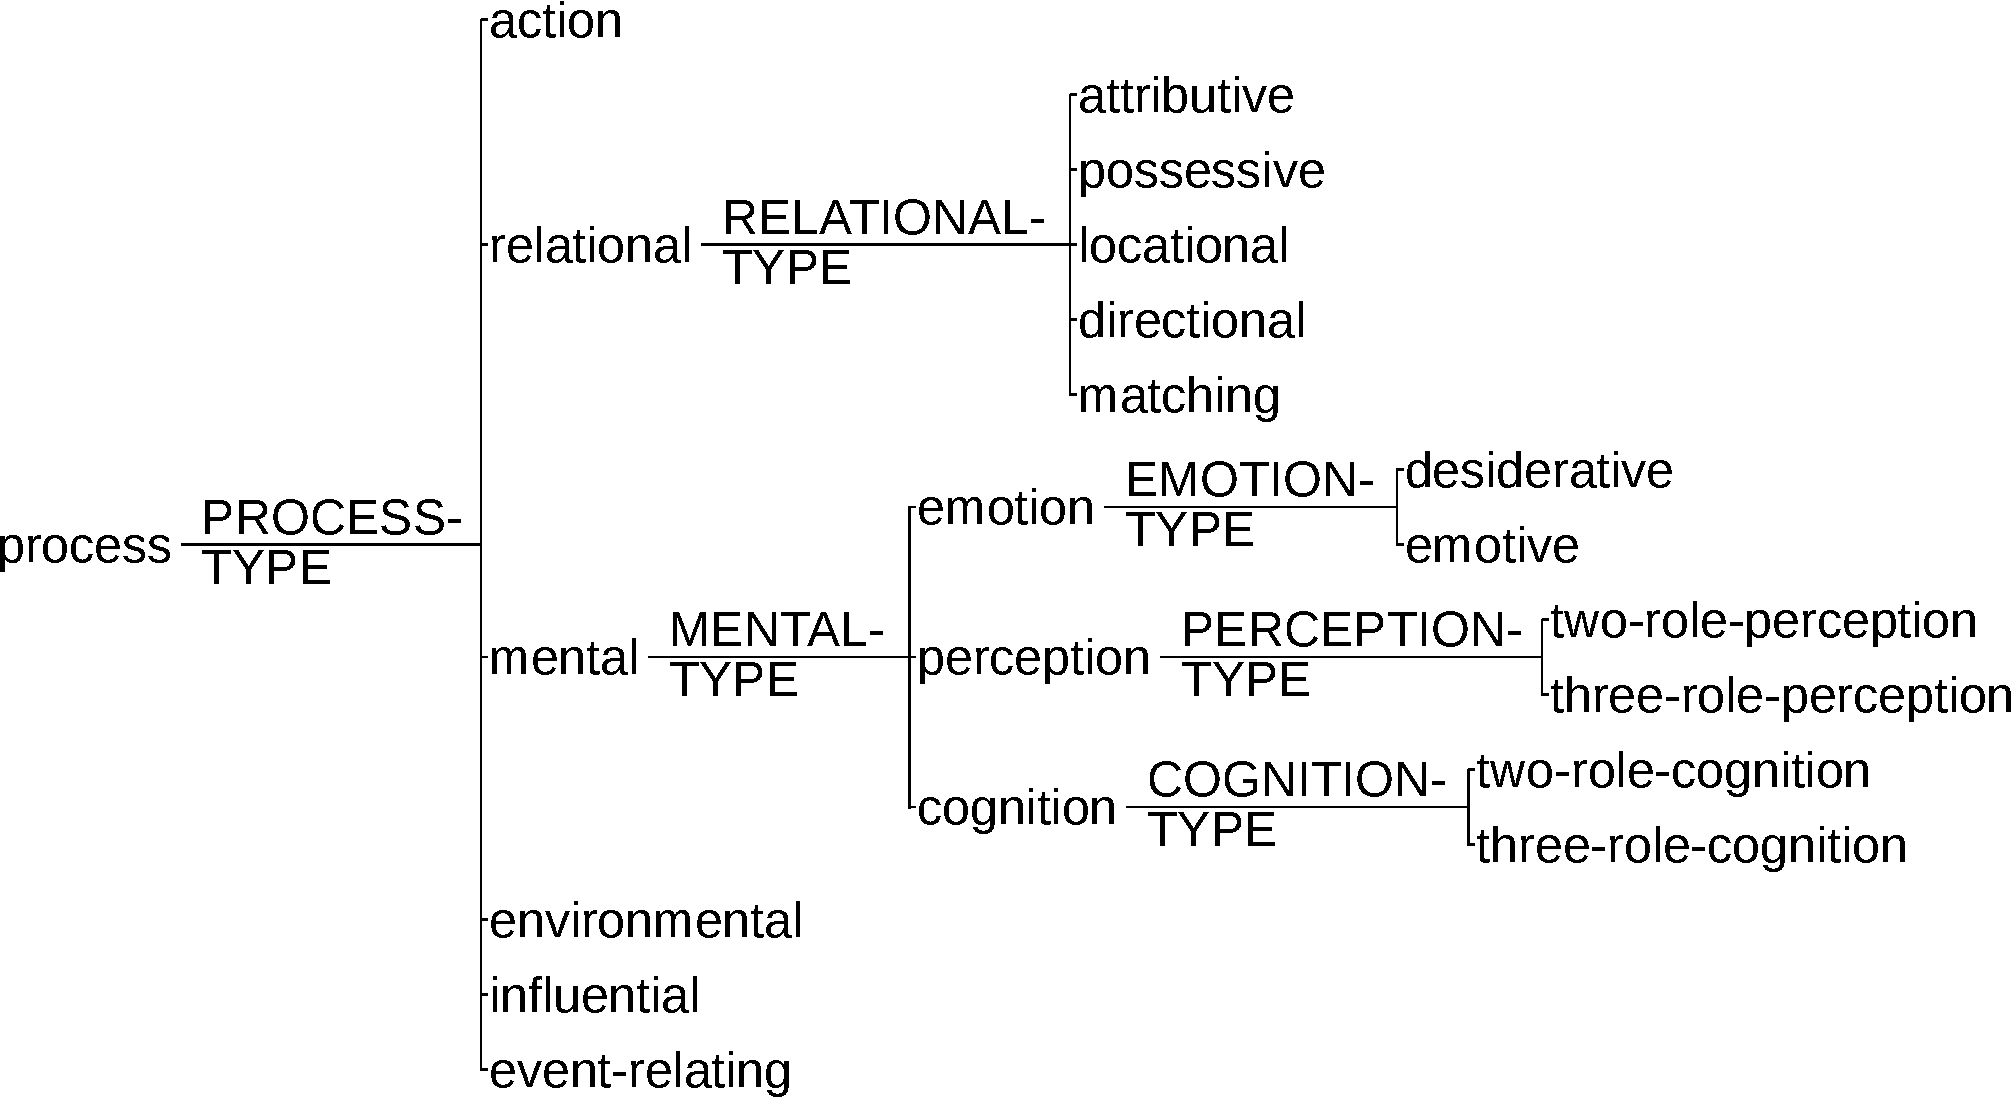
\includegraphics[width=.75\textwidth]{Figures/Evaluation/trans-simplified.pdf}
        \caption{The fragment of the TRANSITIVITY system network that has been used in the corpus}
        \label{fig:transitivity-simplified}
    \end{figure}

    The corpus annotations, developed by Anke Schulz and Tatsiana Markovic \citep[36]{schulz2015me}, cover Cardiff TRANSITIVITY, THEME and MODIFICATION system networks. The grammatical details and the annotation methodology are covered in detail in \citet[48-161]{schulz2015me}. In addition, Schulz provided a set of annotations performed in the same manner for the ``Little Red Riding Hood'' fairy tale comprising 157 clauses which are also included in this evaluation as part of OE corpus.
    
    For the purpose of the current evaluation only the TRANSITIVITY system was considered. The extent to which the system network is covered in the corpus annotations is limited to the top part of the original TRANSITIVITY system network. The used system network fragment is depicted in Figure \ref{fig:transitivity-simplified}, while the whole system network was provided in Chapter \ref{ch:the-grammar}. Employing the entire system network in the annotation process increases in difficulty as the delicacy increases due to the time needed to perform the task \citep[33]{mcenery2006corpus}. The challenge of providing delicate \mbox{(or fine-grained)} corpus annotations using large if not the entire extent of a system network, still has to be addressed in the SFL community at large. 

\subsection{OCD corpus}

     The OCD corpus was created by Ela Oren and myself during a two week scientific mission at the psychology faculty of Tel-Aviv University. The aim of the mission was to design an empirical evaluation for the Parsimonious Vole parser (at that time still under development) using texts consisting of self reports on the challenge of overcoming Obsessive Compulsive Disorder (OCD).
     
     My role was to offer technical support for the annotation tool (UAM Corpus Tool), to prepare the annotation guidelines (provided in \mbox{Appendix \ref{ch:corpus-annotation-methodology}}), present relevant literature and support with the annotation process. Oren selected English texts based on relevance to her research, which was on people recovering from OCD; and after receiving a training in using the UAM Corpus Tool she annotated those texts. The texts represent blog articles of people diagnosed with (OCD), who self-report on the challenge of overcoming OCD. The annotations contain syntactic constituency elements and clause MOOD features. The corpus contains four texts comprising all together 529 clauses and 8605 words. 

    \begin{figure}[!h]
        \centering
        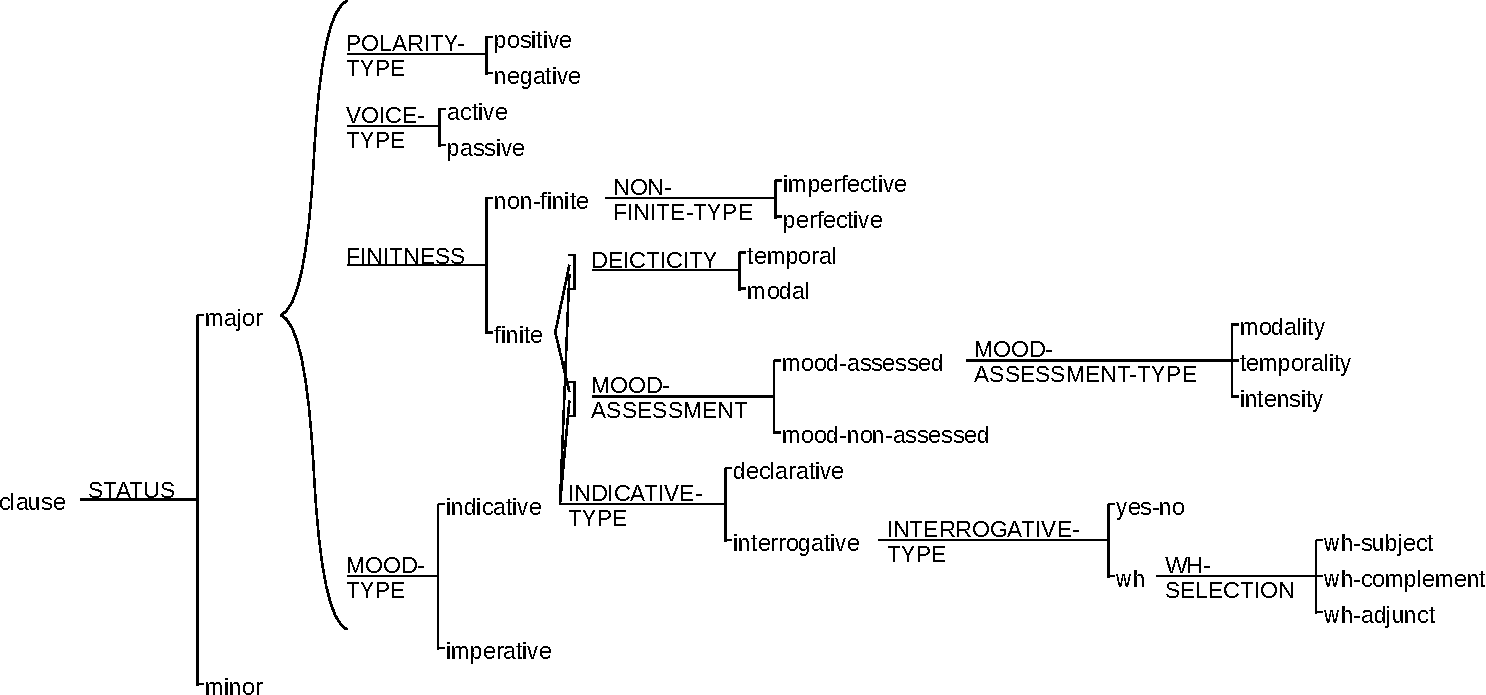
\includegraphics[width=.85\textwidth]{Figures/Evaluation/ocd1-mood-simplified.pdf}
        \caption{The part of the MOOD system network that has been used in OCD corpus annotation}
        \label{fig:mood-ocd-simplified}
    \end{figure}
    
    The corpus annotations account for the main unit classes and the main clause elements. The constituency annotation is based on the Cardiff grammar \citep{Fawcett2008} with some consulting of traditional grammar \citep{Quirk1985} for clarification. The MOOD systemic selections are based on the Sydney grammar \citep{Halliday2013} using the network fragment presented in Figure \ref{fig:mood-ocd-simplified}.
    
    The systemic selections are restricted to the network fragment depicted in Figure \ref{fig:mood-ocd-simplified}. It is a sub-part of the MOOD system network supported by the Parsimonious Vole parser (described in Chapter \ref{ch:the-grammar} and depicted in Figure \ref{fig:clause-mood}). Employing the entire system network in the annotations was difficult because, as the delicacy increases, the time spent for the annotation process increases drastically making the annotation process very tedious and labour intensive \citep{mcenery2006corpus}.
    
\subsection{Differences between corpus annotation and parser output}
\label{sec:differences}

    This section describes the main differences between how the parser structures output and the methodology used to annotate each of the corpora. These differences are mainly due to text normalisation and different treatments of conjunctions and punctuation. In the OCD corpus there are also some segmentation errors as described below.
    
    The Parsimonious Vole parser first normalises the input text before further processing. In this process the tab characters and extra spaces between words are reduced and special characters such as quotes, parenthesis, dashes and other orthographic characters are re-represented in a uniform way. In the OE corpus most of the text is uniformly formatted, but there are few deviations. 
    
\begin{minipage}{\linewidth}
\begin{lstlisting}[numbers=left,basicstyle=\small\tt, stepnumber=1,firstnumber=0,frame=single,caption=Sample of non-normalised raw text from the corpus,label=lst:exampleText,escapeinside={(*}{*)}]
(*\textcolor{black!50}{$_{0}$}*)Red riding hood excerpt(*\textcolor{black!50}{$_{24}$}*)
(*\textcolor{black!50}{$_{25}$}*)"What have you in that basket,   Little Red Riding Hood?"(*\textcolor{black!50}{$_{82}$}*)
(*\textcolor{black!50}{$_{83}$}*)
(*\textcolor{black!50}{$_{84}$}*)"Eggs and butter and cake, Mr. Wolf."(*\textcolor{black!50}{$_{111}$}*)
\end{lstlisting}
\end{minipage}

    Listing \ref{lst:exampleText} presents an example raw text from the annotation dataset containing an initial title line and two sentences separated by an empty line. The greyed index numbers at the beginning and end of each line indicate character offsets. In OE corpus files, the first line plays the role of a header containing the title or the file name and is not considered for annotation or parsing. The extra spaces are eliminated during the normalisation process causing an index shift. 
    
    Before the annotation of the OCD corpus started the normalisation was not at all addressed and so the text contains some irregularities. Mostly it is organised as one sentence per line, but there are instances of extra blank lines or missing new line characters leading to a few sentences per line as a block. The text may also contain tabs and extra blank spaces or blank lines as in Listing \ref{lst:exampleText} at index [82,84]. 

    It is noteworthy to mention that there are segmentation errors in a few cases from the OCD corpus. Some segments are either shifted and include the adjacent spaces (e.g. `` getting this push'' instead of ``getting this push'') or, the converse, leave out one or two characters of a marginal word (e.g. ``the balanc'' instead of ``the balance'').  

    % As mentioned in the beginning of this section, the parser diverges in a few ways from the corpus annotation methodology when it comes to punctuation marks and treatment of conjunctions. Unfortunately there was no time to create a true golden corpus but OCD and OE corpora are close to that. 

    In the OCD and OE corpus annotations, punctuation marks such as commas, semicolons, three dots and full stops are not included in the constituent segments while the parser includes them at the end of each adjacent segment. An example of such a case was provided in Listings \ref{lst:exampleText1} and \ref{lst:exampleText2} in the beginning of this chapter. 
    
    \begin{figure}[!ht]
        \centering
        \begin{subfigure}[b]{0.47\textwidth}
            \centering
            \begin{tikzpicture}[pattern-node]
            \node[pattern-node] (start) {};
            \node[pattern-node, right = 5em of start] (end) {};
            \draw[edge-style] (start) -- (end) node[midway, above]{conjunct 1};
            
            \node[pattern-node, right = .5em of end] (conj) {and};
            
            \node[pattern-node, right = .5em of conj] (start1) {};
            \node[pattern-node, right = 5em of start1] (end1) {};
            \draw[edge-style] (start1) -- (end1) node[midway, above]{conjunct 2};
            
            \end{tikzpicture}
            \caption{Conjuncts annotated as parallel segments}
            \label{fig:segment-conjunction-paralel}
        \end{subfigure}
        \quad
        \begin{subfigure}[b]{0.47\textwidth}
            \centering
            \begin{tikzpicture}[pattern-node] 
            \node[pattern-node] (start) {};
            \node[pattern-node, right =14em of start] (end) {};
            \draw[edge-style] (start) -- (end) node[midway, above]{conjunct 1};
            
            
            \node[pattern-node, below = 0.1em of end] (end1) {};
            \node[pattern-node, left = 8em of end1] (start1) {};
            \draw[edge-style] (start1) -- (end1) node[midway, above]{conjunct 2};
            
            \node[pattern-node, below = -0.6em of start1, xshift=1.8em] (conj) {and};        
            \end{tikzpicture}
            \caption{Conjuncts annotated as subsumed segments}
            \label{fig:segment-conjunction-subsumed}
        \end{subfigure}
        \caption{Treatment of conjunctions in the corpus compared to the parser}
        \label{fig:conjunction-treatment}
    \end{figure}
    
    The treatment of conjunctions that was discussed in Section \ref{sec:coordination} differs as well. In the corpus, the conjunctions (such as ``and'', ``but'', ``so'', etc.) are excluded from the conjunct segments; they are considered markers in the clause/group complexes rather than part of the constituent. The parser, on the other hand, includes the conjunctions into the succeeding adjacent segment. For example, in the corpus we find the segment ``forced me into treatment'' while the parser produces a slightly larger segment ``and forced me into treatment.'' that includes the conjunction at the beginning and the full-stop at the end.
    
    Moreover, the spans of the conjunct segments differ as well due to difference in treatment. Instead of being analysed in parallel, having sibling status as depicted in Figure \ref{fig:segment-conjunction-paralel}, the parser-generated conjunct segments are subsumed in a cascade from the former to the latter as depicted in Figure \ref{fig:segment-conjunction-subsumed}. This is one of the main reasons for long distances between the matched segments when ``conjunct 1'' in Figure \ref{fig:segment-conjunction-paralel} is matched to its counter part ``conjunct 1'' from Figure \ref{fig:segment-conjunction-subsumed}. 
    
    In this section were mentioned the most important aspects by which the corpora annotations and parser output diverge. The evaluation methodology has been developed to take segmentation discrepancies into consideration in order to provide a wider evaluation ground to the systemic associations. The next section explains how this is done.
    
\section{Evaluation methodology}
\label{sec:evaluation-methodology}
    
    This section explains the design of the current evaluation and how it was conducted. I start by explaining how the corpus annotations and the parser output are brought to a common representation as batches of mono-labelled segments. Then I discuss the method to compare the batches of segments in order to find (exact and partial) matches between segments. The matches mean that the parser has produced the same output as in the corpus annotations that is considered to be correct. The number of matched and of non-matched segments is counted for each feature as part of the evaluation data. More details on the method, the matching algorithm and and different types of distance measures that help dealing with partial matches in a controlled manner are presented in Section \ref{sec:alignment-algorithms}.
    
    % Section \ref{sec:differences} described that the matches can be of exact spans and carry the same labels or they can have slightly different spans while still carrying the same labels, meaning that the same linguistic feature is identified in text but it is localised differently. Section \ref{sec:alignment-algorithms} will present an algorithm and different types of distance measurement that help us deal with the exact and partial matches in a controlled manner. 

\subsection{Corpus annotations as a set of mono-labelled segments}

    To compare the segment labels and boundaries we need to understand how they are represented in the annotations and parser output and how they can be brought to a common form comparison. This section explains the UAM Corpus tool representation of the corpus annotations and how are they treated for the purpose of this evaluation.
    
    Both OCD and OE corpora annotations were created with the UAM Corpus Tool \citep{ODonnell2008,ODonnell2008a} version 2.4. They are recorded as segments spanning in the text file from a start to an end index position and the set of features (selected from a systemic network) attributed to that segment. There are no constituency or dependency relations between segments. An example XML representation of an annotation segment is provided in Listing \ref{lst:segment1}. The \textit{id} attribute indicates the unique identification number within the annotation dataset, the \textit{start} and \textit{end} attributes define the segment between two character offsets relative to the beginning of the text file, and the \textit{features} attribute represents all the systemic features attached to this segment (as labels), separated by semicolon. 

\begin{minipage}{\linewidth}
\begin{lstlisting}[language=XML,basicstyle=\small\tt,frame=single,caption=Segment example in UAM corpus tool,label=lst:segment1]
<segment id="4" start="20" end="27" 
features="configuration;relational;attributive" 
state="active"/>
\end{lstlisting}
\end{minipage}

    \begin{figure}[!h]
        \centering
        \begin{subfigure}[b]{0.47\textwidth}
            \centering
            \begin{tikzpicture}[pattern-node]
            \node[pattern-node] (start) {20};
            \node[pattern-node, right = 7em of start] (end) {27};
            \draw[edge-style] (start) -- (end) node[midway, above]{configuration,\\relational,\\attributive};
            \end{tikzpicture}
            \caption{A segment with a set of features}
            \label{fig:segment-multiple}
        \end{subfigure}
        \begin{subfigure}[b]{0.47\textwidth}
            \centering
            \begin{tikzpicture}[pattern-node] 
            \node[pattern-node] (start1) {20};
            \node[pattern-node, right = 7em of start1] (end1) {27};
            \draw[edge-style] (start1) -- (end1) node[midway, above]{configuration};
            
            \node[pattern-node, below = 1em of start1] (start2) {20};
            \node[pattern-node, right = 7em of start2] (end2) {27};
            \draw[edge-style] (start2) -- (end2) node[midway, above]{relational};
            
            \node[pattern-node, below = 1em of start2] (start3) {20};
            \node[pattern-node, right = 7em of start3] (end3) {27};
            \draw[edge-style] (start3) -- (end3) node[midway, above]{attributive};	
            \end{tikzpicture}
            \caption{A set of segments with a single feature each}
            \label{fig:segment-simple}
        \end{subfigure}
        \caption{Example of breaking down a segment with multiple features into multiple segments with a single feature}
        \label{fig:segment-breackdown}
    \end{figure}

    In order to provide the possibility of evaluating each feature in a simple and transparent fashion, the annotation segments are constrained to carry only one label each. This means that the representation employed by the UAM corpus tool, with multiple labels per segments, as depicted in Figure \ref{fig:segment-multiple}, is not suitable as such and needs an adaptation. When it is read from the input, the segments with multiple features are broken down into multiple segments (over the same index span) for each feature in the original segment, as depicted in Figure \ref{fig:segment-simple}. Doing so permits the evaluation to focus on one or a set of features by freely and conveniently selecting only the segments that contain exactly those features.
    
    The representation of the parser output, to be suitable in the current evaluation, needs a similar adaptation. In the next section I present how this is done. 

\subsection{Parser output as a set of mono-labelled segments}
% todo update the section start
    
    In order to compare the parser output to the corpus segments they need to be turned into the same form. In this section, I describe the task of turning rich constituency graphs (CG) into labelled segments similar to those from the corpus presented in the previous section. 
    
    To make the parser output segments comparable to the ones in the corpus they need to refer, in terms of their offsets and indexes, to the same raw text. This is not the case for two reasons. First, the parser identifies sentence boundaries and then processes them one sentence at a time. This means that the original input text is chunked based on punctuation and the indexes are reset for each sentence. Correspondingly the parser output is produced with respect to the new indexes. Second, the text after being chunked is normalised. This means that the word indexes are readjusted within the sentence text and is directly reflected in the parser output. Before the evaluation can take place the parser output segments need to be re-indexed with respect to the original raw text. 
    
    To fulfil this task, the text processed by the parser is re-indexed back into the original raw text at the level of words (tokens), constituents and sentences. Algorithm \ref{alg:re-index-text} provides pseudo-code of the re-indexing process.
     
    \begin{algorithm}[!ht]
        \Input {CG bundle, \text} %, \dg
        \Begin {
            offset $\leftarrow$ 0\;
            \For{\cg \KwTo CG bundle}
            {
                generate segments for \cg indexed on \text given the offset\;
                offset $\leftarrow$ the end of \cg\;
            }
        }
        \caption{Sentence level re-indexing of CG according to the raw text}
        \label{alg:re-index-text}
    \end{algorithm}

    Section \ref{sec:creation-constituency-graph} explained that the parser processes one sentence at the time. If more than one sentence is provided as input text, then the produced output is not only one but a set of constituency graphs. This is reflected in the input for Algorithm \ref{alg:re-index-text} which is the array of CGs produced by the parser and the original text. The result of this algorithm is a set of mono-labelled segments indexed according to the raw text, just as the corpus annotations. 
    
    This task is performed by sequentially iterating the array of output constituency graphs and re-indexing each of them with respect to the offset calculated after the re-indexing its predecessor. The process of re-indexing a CG structure is presented in Algorithm \ref{alg:re-index-words-and-cg}. The returned result is a set of segments from the constituency graph considering a given offset.

    \begin{algorithm}[!ht]
        \Input {\cg, \text, sentence offset} %, \dg
        \Begin {
            words $\leftarrow$ get \cg the list of words \;
            \For{\word \KwTo list of sentence word segments}
            {
                find the \word in the \text after a given sentence offset\;
                \eIf{\word found}
                {
                    start $\leftarrow$ get first word start index\;
                    end $\leftarrow$ get the last word end index\;
                    create a new segment (start, end, \word)\;                
                }
                {
                    generate a warning (manual adjustment needed)\;
                }
            }
            \For{\node \KwTo \cg in BFS postorder}
            {
                find the word span of the constituent\;
                start $\leftarrow$ get first word start index\;
                end $\leftarrow$ get the last word end index\;
                labels $\leftarrow$ get \node class, function and features\;
                create new segment (start, end, labels)\;
            }
            \Return set of segments\;
        }
        \caption{Constituent level re-indexing at the level of constituents according to the raw text}
        \label{alg:re-index-words-and-cg}
    \end{algorithm}

    In Algorithm \ref{alg:re-index-words-and-cg}, the indexing is performed first at the word (token) level. At the same time the mono-labelled segments are generated for each token. Then the CG constituent nodes that are group or clause rank are re-indexed based on constituents below them, i.e. words that have just been re-indexed in the step before. The indexes of the constituent segments are set to be the beginning of the first word and the end of the last word. The labels assigned to the segments are the constituent unit class, function(s) and all the systemic features. As the segments can carry a single label only then for every feature, function and unit class a new segment is created. This is in line with the practice described above concerning usage of mono-labelled segments.

    Now that I have shown how the parser output is aligned to the original text in the corpus and is represented as a set of mono-labelled segments, it is possible now to compare the parser output and the corpus annotations in order to asses the parser accuracy. The next section explains how this is done. 

\subsection{Segment alignment method and evaluation data}
\label{sec:alignment-algorithms}    

    Both the corpus annotations and the parser output are represented as a set of mono-labelled segments on the raw corpus text and can be compared to evaluate the parser accuracy. This section explains how this comparison is done. I first present a strict method of evaluation and then introduce a more permissive/tolerant  method of evaluation based on segment similarity and distance measurements. 

    First, a straight-forward evaluation method is to check for a perfect match between every segment in the parser output and a corresponding segment in the corpus annotations. A perfect match means that each parser segment has a counter part in the corpus annotations whose start index, end index and label are equal. This signifies that the parser generated segment is correct.
    
    Using this method of evaluation the resulting data contain the counts of (a) how many segments with the same label are matching, (b) how many corpus segments are not matching and (c) how many parser segments are left unmatched. Then the data is aggregated for each label in the corpus annotation and parser output combined. 
    
    In Section \ref{sec:differences} I presented some differences between the parser output and the corpus annotations. Most of these differences are comparable especially in that they manifest as slight variations in the segment spans, i.e. shifted start and/or end segment index, while the segment labels are exactly the same. The above presented method is not satisfactory for the current evaluation because by design it leaves out about (20\%) of valuable partial matches. I present next an alternative evaluation approach where I address how the differences between segments can be judged in an objective controlled manner.
    
    A simple metric for the difference between the segments taking into account their start and end indexes is that of \textit{geometric distance}. For two segments $S(start_S,end_S)$ and $T(start_T,end_T)$ the geometric distance is defined in Equation \ref{eq:distance}. We can replace the difference between start and end indexes with $\varDelta_{start}$ and $\varDelta_{end}$ notation and obtain the reduced form provided in Equation \ref{eq:distance-simpliefied}. This distance metric penalises errors in proportion to the length difference and the shift between segments. 
    
    \begin{equation} \label{eq:distance}
    d= \sqrt{(start_S - start_T)^{2}+(end_S-end_T)^{2}}
    \end{equation}
    
    \begin{equation} \label{eq:distance-simpliefied}
    d= \sqrt{\varDelta_{start} ^{2}+\varDelta_{end}^{2}}
    \end{equation}
    
    Accounting for differences in the segment spans is a well known task in mainstream computational linguistics called \textit{text segmentation evaluation}. A variety of segmentation evaluation metrics have been proposed among which the most known are $P_k$ \citep[198--200]{beeferman1999statistical}, \textit{WindowDiff} \citep[10]{pevzner2002critique}, \textit{Segmentation Similarity} \citep[154-156]{fournier2012segmentation} and \textit{Boundary Edit Distance} \citep{fournier2013evaluating}. Each of these metrics have been shown to have strengths and flaws. For example both $P_k$ and $WindowssDiff$ under-penalise errors \citep{lamprier2007evaluation} and have a bias towards favouring segmentation with few or tightly-clustered boundaries \citep{niekrasz2010unbiased}, while segmentation similarity tends to overly optimistic values due to its normalisation \citep{fournier2013evaluating}. Based on the evaluation data, these distances will be further discussed in Section \ref{sec:segmentation-evaluation}. 
    
    % All the above metrics take into account that the content of the segment text may vary and so they use text edit distance to account for that. In the case of the current evaluation the segments are defined on the same text and thus only the segment indexes are relevant. 

    Now that the metrics for comparing segments have been introduced I move on to present the second evaluation method, which, in addition to accounting for the exact matches, accounts for close matches between segments using the distance measurements presented above. 
    
    The second evaluation method is to align two sets segments taking into consideration exact and partially matching pairs. This task is similar to the well known problem in computer science called the \textit{stable marriage problem} \citep{Gusfield1989}. I adopt here the computer science framing of the problem to explain the second evaluation method.
    
    The standard enunciation of the stable marriage problem is provided below and is solved in an efficient algorithm named Gale-Shapley \citep{Gale1962}.
    
    \begin{quotation}
        Given \textit{n} men and \textit{n} women, where each person has ranked all members of the opposite sex in order of preference, marry the men and women together such that there are no two people of opposite sex who would both rather have each other than their current partners. When there are no such pairs of people, the set of marriages is deemed stable \citep{iwama2008}.
    %    \footnote{see \href{https://en.wikipedia.org/wiki/Stable_marriage_problem}{stable marriage problem on Wikipedia}}
    \end{quotation}

    In the context of this evaluation the group of men is associated with the segments generated automatically by the parser and the group of women with the segments available from the manual analysis. 

    The standard stable marriage problem is formulated such that there is a group of men and a group of women and each individual from each group expresses their preferences for every individual from the opposite group as an ordered list. The assumption is that the preferences of every individual are known and expressed as a complete ordered list of individuals from the opposite group ranging from the most to the least preferred one. Thus the preference list must be \textit{complete} and \textit{fully ordered}. 

    % \noindent
    % \begin{minipage}{\textwidth}
    \begin{algorithm}[!ht]\small
        \Input{\aslist, \mslist} %, \dg
        \Begin{
            mark all \aslist and \mslist free\;
            compute distances from each \mslist to every \aslist\;
            \While{exist free segments in \aslist}{
                \as $\leftarrow$ first free segment from \aslist\;
               \If{exist in \mslist un-compared segment to \as}{
                   \ms $\leftarrow$ the nearest among \mslist to \as with identical label \;
                   \If{\ms is free}{
                       match \as and \ms \;
                       mark \as and \ms as non-free \;
                   }               
               \Else{
                       $\as'$ $\leftarrow$ the current match of \ms \;
                       \If{\as is closer to \ms than $\as'$}{
                           match \as and \ms \;
                           mark \as and \ms as non-free \;
                           mark $\as'$ as free \; 
                       }
                   }
               }
               \Else{
                   mark \as as non-free and non-matching 
               }
            }
        }
        \caption{The algorithm for matching parser and corpus segments}
        \label{alg:matching}
    \end{algorithm}
    % \end{minipage}

    Algorithm \ref{alg:matching} represents a modified version of Gale-Shapley algorithm. In the process each parser segment is attempted to match with the closest corpus segment. A match is established if there is no another parser segment that is even closer to the candidate corpus segment. The remaining corpus and parser segments are marked as non-matching.

    Using this method of evaluation we can count for every distinct label (a) how many segments match perfectly, i.e. the distance is zero, (b) how many segments partially match, i.e. the distance is greater than zero, (c) how many corpus segments are unmatched and (d) how many parser segments are unmatched. Hence, we get a four frequency counting numbers per label for each label used in the corpus annotation and parser output combined. These frequency numbers are used to compute parser accuracy metrics. Furthermore, the partial matches can be analysed to estimate the degree of the deviation and derive insights what can be done about it.  

\section{Evaluation of syntactic structure generation}
\label{sec:syntactic-evaluation}
    
    Having presented the evaluation method, I further proceed with presenting the evaluation results in two parts: the first part focuses on the syntagmatic aspects and the second part deals with paradigmatic aspects of the parser output. In this section, I present the evaluation results for the parser accuracy to generate the syntagmatic aspects of an SFL analysis (described in Chapter \ref{ch:parsing-algorithm}). The discussion of evaluation results covers the accuracy of parser segmentation, the distribution of distances among the matched segments, and the accuracy to detect the main unit classes and clause main Mood and Transitivity elements. 
    
\subsection{Segmentation evaluation}
\label{sec:segmentation-evaluation}
    
    This section presents the evaluation data on text segmentation. As we will see below, over 60\% of the parser segments coincide with the corpus segments. The differences, which were described in Section \ref{sec:differences}, are mainly due to differences in annotation approach, text normalisation and some segmentation errors in the OCD annotations (e.g. missing or including some extra characters). 
    
    The segmentation counts are provided in Table \ref{tab:segmentation-stats}. The columns represent  the number of matched segments, the segments from the corpus that have not been matched and the parser output segments left unmatched. There are 6665 segments that perfectly align and 11073 segments that align partially or completely. %This means that the exact matched are included into the latter along with other 5000 partially matching segments. 
    
    \begin{table}[!ht]
    \centering
    \begin{tabular}{lccc}
    \toprule
    {} &  Matched &  Corpus non-matched &  Parser non-matched \\
    \midrule
    Exact matches only &     6665 &                1319 &                4332 \\
    Exact and close matches &    11073 &                1319 &                4332 \\
    \bottomrule
    \end{tabular}
    \caption{Count statistics of matched and non-matched segments}
    \label{tab:segmentation-stats}
    \end{table}
    
    
    \begin{table}[!ht]
    \centering
    \begin{tabular}{lccc}
    \toprule
    {} &  Precision &  Recall &   F1 \\
    \midrule
    Exact matches only &        0.61 &    0.83 & 0.71 \\
    Exact and close matches                &        0.72 &    0.89 & 0.80 \\
    \bottomrule
    \end{tabular}
    \caption{Segmentation accuracy}
    \label{tab:segmentation-accuracy}
    \end{table}
    
    The statistics provided in Table \ref{tab:segmentation-stats} translate into precision, recall and $F_1$ scores as provided in Table \ref{tab:segmentation-accuracy}. The parser segmentation accuracy is 71\% for exactly matching segments and 80\% for partially matching ones. The distances between segments are measured in several ways. Next follows an analysis of these measurements. 
    
    The segmentation differences are measured, as introduced in Section \ref{sec:evaluation-methodology}, using several distance metrics: (a) geometric (Euclidean) distance, (b) edit (Levenshtein), (c) generalised hamming distance (GHD) \citep{Bookstein2002}, $P_k$ \citep[198--200]{beeferman1999statistical}, \textit{WindowDiff} \citep[10]{pevzner2002critique}. 
    The data is calculated on a number of over 12500 segment pairs out of which 62\% are exact matches and 38\% are close matches. 
    
    Before providing the interpretations to the data, I first show it is sufficient to discuss two of these distances as the other ones are strongly correlated to them and thus can be omitted from the discussion. Table \ref{tab:correlation-matrix-distances} represents the Pearson correlation matrix for the distance types. 
    
    \begin{table}[!ht]
    \centering
    \resizebox{\textwidth}{!}{%
    \begin{tabulary}{\textwidth}{lccCcc}
    \toprule
    {} &  Levinstein &  Geometric &  Generalised Hamming &   Pk &  WindowDiff \\
    \midrule
    Levinstein          &        1.00 &       0.99 &                 0.53 & 0.45 &        0.54 \\
    Geometric           &        0.99 &       1.00 &                 0.52 & 0.45 &        0.54 \\
    Generalised Hamming &        0.53 &       0.52 &                 1.00 & 0.84 &        0.92 \\
    Pk                  &        0.45 &       0.45 &                 0.84 & 1.00 &        0.92 \\
    WindowDiff          &        0.54 &       0.54 &                 0.92 & 0.92 &        1.00 \\
    \bottomrule
    \end{tabulary}
    }
    \caption{Pearson correlation coefficients for pairs of distance measure types}
    \label{tab:correlation-matrix-distances}
    \end{table}
    
    The Pearson correlation coefficient measures the direction and strength of a linear correlation between two variables. In this case, the variables are distance types. The standard interpretation for this coefficient is as follows. A coefficient value between 0.1 and 0.3 indicated a weak linear relationship between the variables. If it is between 0.3 and 0.5 the relation is moderate, between 0.5 and 0.7 it is strong; and a score over 0.7 indicates a very strong correlation of variables. 
    
    Using the above interpretation we can partition the correlation matrix into two groups of strongly correlated variables. At the same time both groups are only moderately (\textasciitilde50\%) correlated to each other. The Levinstein and Geometric distances are nearly identical with a 99\% correlation though from this point on I will exclude the Levinstein distance and employ the geometric distance only as representative for both. 
    
    The generalised Hamming distance, $P_k$ and WindowDiff bear a strong correlation of 92\% to WindowDiff. I exclude, from now on, $P_k$ and generalised hamming distance from further discussions and use WindowDiff as the representative of the three distances. This choice is also based on the fact that WindowDiff was proposed to overcome weaknesses of $P_k$ \citep[10]{pevzner2002critique}.
    
    Above, I have shown that the geometric distance and WindowDiff distance are the significant measures of distance in this segmentation evaluation. Next, I provide descriptive data (in Table \ref{tab:distance-descriptions}) and offer interpretations for each of them.
    
    \begin{table}[!ht]
    \centering
    \resizebox{\textwidth}{!}{%
    \begin{tabulary}{\textwidth}{LccccRcc}
    \toprule
    {} &  Min &    Max &  Mean &   SD &  Rel SD &  Skewness &  Kurtosis \\
    \midrule
    Levinstein          & 0.00 & 219.00 &  5.37 & 15.99 &          2.98 &  5.57 &     42.63 \\
    \textbf{Geometric}           & 0.00 & 219.00 &  4.99 & 14.67 &          2.94 &  5.56 &     43.14 \\
    Generalised Hamming & 0.00 &   8.00 &  1.84 &  2.87 &          1.56 &  1.30 &      0.09 \\
    Pk                  & 0.00 &   1.00 &  0.18 &  0.29 &          1.62 &  1.40 &      0.57 \\
    \textbf{WindowDiff}          & 0.00 &   0.86 &  0.15 &  0.23 &          1.59 &  1.32 &      0.28 \\
    \bottomrule
    \end{tabulary}
    }
    \caption{Descriptive statistics for each set of distance measurements between corpus and parser segments}
    \label{tab:distance-descriptions}
    \end{table}

    Table \ref{tab:distance-descriptions} presents the descriptive statistics (columns) for every distance type (rows). The first three columns provide min, max and mean (M) values. The \textit{SD} column means \textit{standard deviation} while the \textit{Rel SD} represents \textit{relative standard deviation}  (or coefficient of variation). The Skewness and Kurtosis are the last statistical indicators for describing the distance distribution, which I will explain below.
    
    The relative standard deviation is the ratio between the standard deviation and mean value, i.e. (SD/M) and measures how concentrated the data is around the mean: the more concentrated, the smaller the standard deviation. It is considered that a relative standard deviation between 0 and 0.5 indicates tightly clustered data around the mean; if it is situated between 0.5 and 1 then it means the data is more spread out; if, however the value is over one then it means the data is very scattered. 
    
    \begin{figure}[!ht]
    \centering
    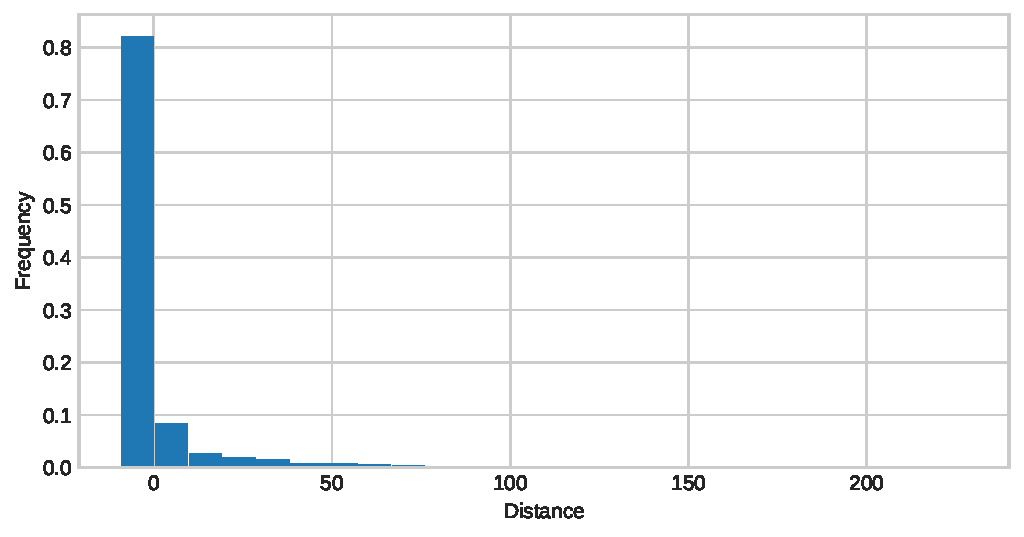
\includegraphics[width=.85\textwidth]{evaluation-results/figures/distance-distribution-histogram-Geometric-25.pdf}
    \caption{Matched segments geometric distance distribution histogram (binning=25)}
    \label{fig:distance-distribution-histogram-Geometric-25}
    \end{figure}

    In the current evaluation, the geometric distance between corpus and parser segments spans from a minimum 0 to maximum 219 characters. The mean distance is 4.99, which is close to the minimum point, with a standard deviation of 14.67 (deviation of almost 30 times the mean). The skew over 1, in this case 5.56, indicates a strong asymmetry to the right, and the kurtosis of 43.14 (almost 15 times the threshold of 3) indicates that most of the data, about 80\%, gravitate towards the left, between 0 and slightly over the mean, while the rest of the data point continue into a very long tail to the right. This is depicted in Figure \ref{fig:distance-distribution-histogram-Geometric-25}. 
    
    \begin{figure}[!ht]
    \centering
    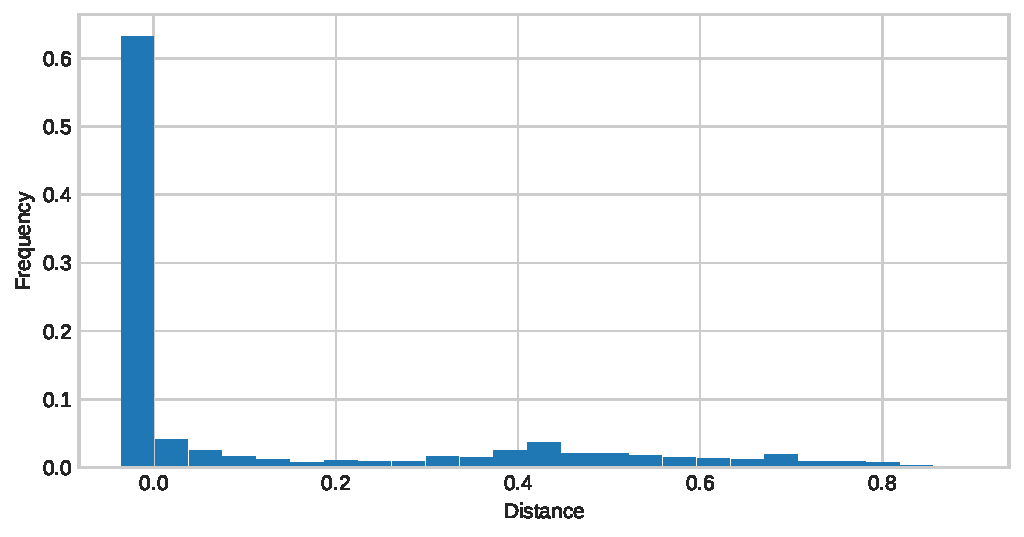
\includegraphics[width=.85\textwidth]{evaluation-results/figures/distance-distribution-histogram-WindowDiff-25.pdf}
    \caption{Matched segments WindowDiff distance distribution histogram (binning=25)}
    \label{fig:distance-distribution-histogram-WindowDiff-25}
    \end{figure}
    
    As appears in Figure \ref{fig:distance-distribution-histogram-Geometric-25}, the data does not follow a normal but a power law distribution \citep{newman2005power}. This means that 62\% of the segments are not shifted at all and 83\% of the segments are slightly shifted up to 5 characters. The rest (17\%) of the segments are shifted by more than 5 characters. These ratios approximate Patetto 80-20 distribution law but may as well fit Zipf's law \citep{newman2005power}. In future work, properties of these data should further be analysed, including the distribution fitting, that is selection of the theoretical distribution that fits best this dataset.
    
    The next distance measure that I discuss is WindowDiff distance between corpus and parser segments. One crucial difference to geometric distance is the normalisation to a [0,1] interval. In the current evaluation, the WindowDiff distance distribution, depicted in Figure \ref{fig:distance-distribution-histogram-WindowDiff-25}, spans from a minimum 0 to maximum score of 0.86. The mean distance is 0.15 with a standard deviation of 0.23. The mean value is close to the minimum point, the relative standard deviation of 159\%, the skew over 1 indicates a strong asymmetry to the right, and the kurtosis of 0.28 indicate the distribution does not have many outliers in the tail. These parameter values are similar to those of the geometric distance but to a lesser degree. 
    
    One positive aspect of WindowDiff distance distribution is that the tail is not so long due to its normalised structure. This results in aggregation of the outliers we have observed in geometric distance distribution into a compact spectrum. This way, diminishing the kurtosis below 3, which no longer indicates an abnormally long tail to fit a normal distribution. 
    
    The histogram in Figure \ref{fig:distance-distribution-histogram-WindowDiff-25} also resembles a power law distribution and more analysis work needs to be done in the future, including the distribution fitting and relation to the causes of partial matches in the first place. 
    
    This section presented the segmentation evaluation. The data shows that the parser generates exact segments as provided in the corpus with an accuracy of 0.71 $F_1$ score, and segments that partially correspond to those in the corpus with an accuracy of 0.8 $F_1$ score. The distances of the partially matched segments, in about 83\% of the cases do not exceed 5 characters, but can span, most probably by mistake, over 200 characters in less than 17\% of cases. Next I present the evaluation of the label assignments for the segments corresponding to constituency units, i.e. (unit) classes and functions.

\subsection{Unit class evaluation}
\label{sec:unit-class-evaluation}
    In this and the next section I present the parser syntactic accuracy. It aims to measure, in this section, how well the main unit classes, and in the next sections, the clause main elements have been generated by the parser compared to the corpus. The unit class evaluation is performed on the OCD corpus. This evaluation comprises the following unit classes: clause and nominal, prepositional, adverbial and adjectival groups. No clause complexes, group complexes or word types are included. The evaluation data is depicted in Figure \ref{fig:unit-types-data}. The names of the unit classes are provided on the \textit{x} axis at the bottom of the graph while on the \textit{y} axis the absolute number of occurrences is provided. 
    
    The meaning of exact and close match has been explained in Section \ref{sec:segmentation-evaluation} and from now on the label ``Matched'' will mean the segments that are either exactly or closely matched all together, while the label with a remark ``(exact only)'' means that it applies to only the portion of the exactly matched segments. 
    
    
    \begin{figure}[!ht]
    \centering
    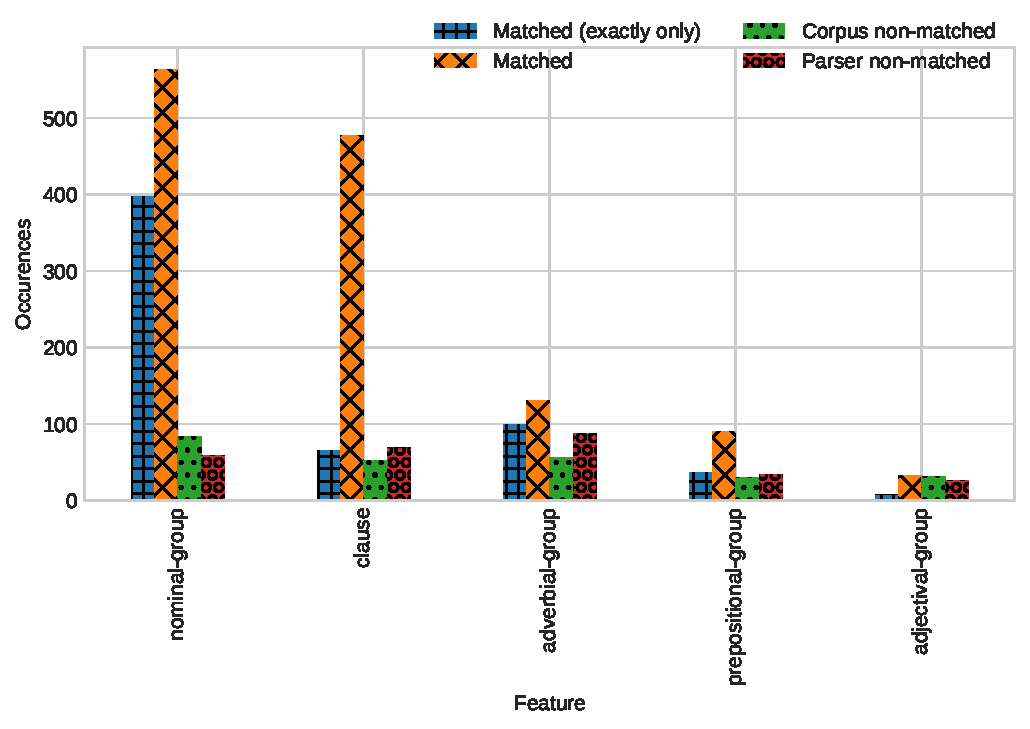
\includegraphics[width=.85\textwidth]{evaluation-results/figures/unit-types-data.pdf}
    \caption{Bar chart of matched and non-matched segments for the main unit classes}
    \label{fig:unit-types-data}
    \end{figure}
    
    To make the data easier to read and interpret I present the evaluation data in a table form using relative values to the number of matched segments. The absolute values of the evaluation statistics are contained in the graphical form and also available in the appendices in the table form. The relative evaluation data in this and the following sections will be presented in tables with the same structure. Using Table \ref{tab:unit-types-relative} as example, the column meaning is as follows. The first column contains the name of the unit class, element or feature. The column ``Matched'' contains the absolute number of matched segments with a specific label. The three other columns represent the number of segments relative to the ``Matched'' ones. So the column ``(\%) Matched (exactly only)'' means that out of all the matched segments that many represent exact matches and the rest up to 100\% are partially matched segments. The column ``(\%) Corpus non-matched'' represent the number of segments relative to the total number of segments of particular type in the corpus, which remain unmatched. %The column signifies the fraction of segments that remain unmatched, while the rest up to 100\% have, each, a corresponded in the parser output. 
    The column ``(\%) Parser non-matched'' represents the number of segments (relative to the total number of segments of particular type in the parser output) in the parser output that do not have a correspondent in the corpus.
    
    \begin{table}[!ht]
    \centering
    \begin{tabulary}{\textwidth}{lCCCC}
    \toprule
    {} &  Matched &  (\%) Matched (exactly only) &  (\%) Corpus non-matched &  (\%) Parser non-matched \\
    \midrule
    nominal-group       &   564.00 &                       70.39 &                   12.96 &                    9.47 \\
    clause              &   477.00 &                       13.84 &                    9.83 &                   12.64 \\
    adverbial-group     &   131.00 &                       76.34 &                   29.95 &                   40.18 \\
    prepositional-group &    90.00 &                       41.11 &                   25.00 &                   27.42 \\
    adjectival-group    &    33.00 &                       24.24 &                   49.23 &                   44.07 \\
    \bottomrule
    \end{tabulary}
    \caption{The evaluation statistics relative to the number of matched segments for the main unit classes}
    \label{tab:unit-types-relative}
    \end{table}
    
    The evaluation data from Table \ref{tab:unit-types-relative} indicate that most (over 70\%) of the nominal and adverbial groups are identified with the exact same borders as in the corpus while clause borders exhibit the most disagreement reflected by their low score of exact matches, only 13.84\%. The proportion of unmatched unit class segments in both the corpus and parser output varies between 9\% for clauses and nominal groups, and over 40\% for adjectival and adverbial groups. These proportions, however, are better interpreted when they are embedded into precision and recall score, which are provided in Table  \ref{tab:unit-types-combined-F1}. 
    \begin{table}[!ht]
    \centering
    \begin{tabular}{lcccccc}
    \toprule
     & \multicolumn{3}{c}{Exact match only} & \multicolumn{3}{c}{Exact and close match} \\ \cline{2-7} 
     & Precision & Recall & F1 & Precision & Recall & F1 \\ 
    \midrule
    nominal-group & 0.87 & 0.83 & 0.85 & 0.91 & 0.87 & 0.89 \\
    adverbial-group & 0.53 & 0.64 & 0.58 & 0.87 & 0.90 & 0.89 \\
    prepositional-group & 0.52 & 0.55 & 0.54 & 0.73 & 0.75 & 0.74 \\
    clause & 0.49 & 0.56 & 0.52 & 0.60 & 0.70 & 0.65 \\
    adjectival-group & 0.24 & 0.20 & 0.22 & 0.56 & 0.51 & 0.53 \\ 
    \bottomrule
    \end{tabular}
    \caption{Parser accuracy statistics for for the main unit classes}
    \label{tab:unit-types-combined-F1}
    \end{table}
    
    The scores provided in the first three columns are calculated with respect to exact matches only and the last three columns with respect to all the matches. This can be seen reflected in the lower precision, recall and $F_1$ scores when compared to their correspondents in the last three columns. The exact match scores, nonetheless, constitute an appropriate baseline for the parser. Note that in all cases of a match, close or exact, the segments bear the same label, and so, as explained in Section \ref{sec:differences}, the source of the divergence is mainly in the segment index span. 
    
    The last three columns in Table \ref{tab:unit-types-combined-F1} show that clause and normal group units are identified with almost 0.9 $F_1$ measure, which is an encouraging result, while the adjectival and adverbial groups score 0.53 and 0.65 indicates that there is some space for improvement. 
    Further investigation is needed to discover the reason for the lower scores as there seems to be no obvious cause other than corpus and/or parser errors. There may possibly be errors in the corpus because it has been annotated by a single annotator which may be unreliable. Also, as visible in Figure \ref{fig:unit-types-data}, there is a contrast in the number of segments between the first two unit types and the last three with a ratio of one to four or more. The lower number of exemplars (close to and below 100) in this evaluation contributes, to a certain extent, to the lower accuracy statistics.
    
\subsection{Clause Mood elements evaluation}
\label{sec:unit-mood-element-evaluation}

    In this section I describe the evaluation statistics reflecting the parser capacity to identify the main elements of a clause. The data available in the corpus unfortunately does not permit us to evaluate elements of the lower rank units such as nominal, prepositional, adjectival and other groups. Next, I present statistics on the clause Mood elements, which were described in Chapter \ref{ch:the-grammar}. These elements are present in the annotations of the OCD corpus as explained in the beginning of this chapter in Section \ref{sec:corpus}. 
    
    \begin{figure}[!ht]
    \centering
    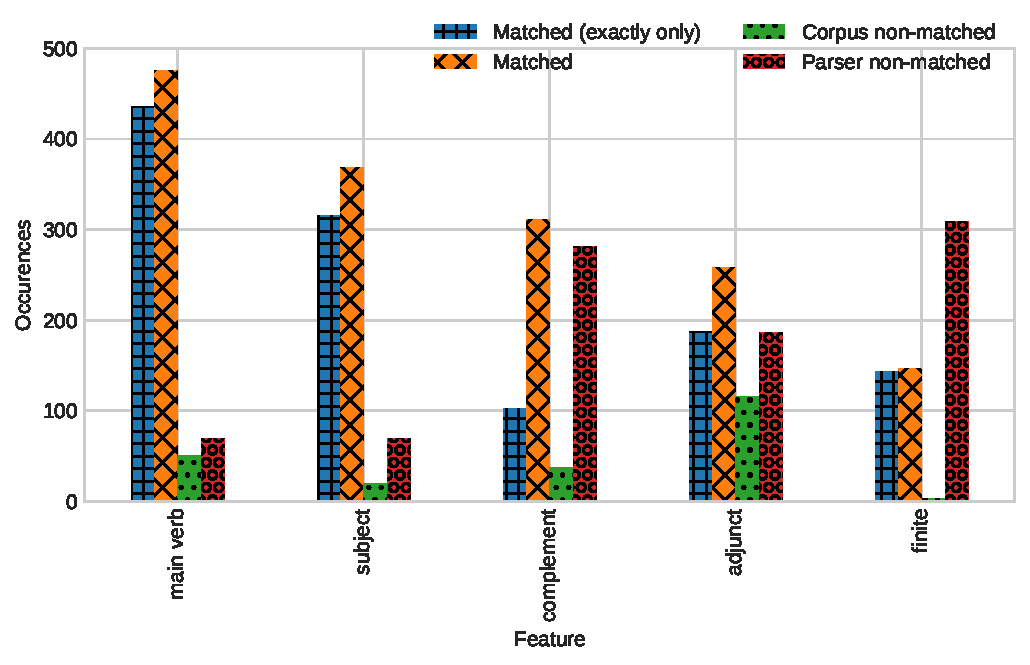
\includegraphics[width=.85\textwidth]{evaluation-results/figures/unit-elements-mood-data.pdf}
    \caption{Bar chart of matched and non-matched segments for the clause main Mood elements}
    \label{fig:unit-elements-mood-data}
    \end{figure}
    
    The OCD corpus annotations provide the main syntactic (Mood) elements in the clause. Some of them, such as Auxiliary verbs, Main verb extension, Negation particle, and others have been omitted in the corpus annotation and are thus missing in the present evaluation. Figure \ref{fig:unit-elements-mood-data} reflects the absolute values from the empirical data. 
    
    The parser accuracy measurements for the main syntactic functions are contained in Table \ref{tab:unit-elements-mood-combined-F1}. The $F_1$ score for subjects and main verbs is nearly 0.9 while the complements and adjuncts are over 0.6. Finite element scores nearly 0.5 which is surprisingly low for this element. The reason for this lays in the incomplete corpus annotations. In the annotation process the conflated Finite and Main verb elements were not distinguished. So, when there was a main verb that was also a finite, only the main verb function was marked, which is incomplete by SFL standards. This incompleteness is clearly reflected in the contrast between low precision of 0.32 and high recall of 0.98. 
    
    \begin{table}[!ht]
    \centering
    \begin{tabular}{lcccccc}
    \toprule
     & \multicolumn{3}{c}{Exact match only} & \multicolumn{3}{c}{Exact and close match} \\ \cline{2-7} 
     & Precision & Recall & F1 & Precision & Recall & F1 \\ 
    \midrule
    main verb & 0.86 & 0.90 & 0.88 & 0.87 & 0.90 & 0.89 \\
    subject & 0.82 & 0.94 & 0.88 & 0.84 & 0.95 & 0.89 \\
    complement & 0.27 & 0.73 & 0.39 & 0.53 & 0.89 & 0.66 \\
    adjunct & 0.50 & 0.62 & 0.55 & 0.58 & 0.69 & 0.63 \\
    finite & 0.32 & 0.98 & 0.48 & 0.32 & 0.98 & 0.49 \\
    \bottomrule
    \end{tabular}
    \caption{Parser accuracy statistics for the clause main Mood elements}
    \label{tab:unit-elements-mood-combined-F1}
    \end{table}
    
    The number of complements unmatched in the parser output is nearly the same as the number of matched complements. This is reflected in the 0.53 precision score and nearly 0.9 recall rate which overall lead to an $F_1$ score lower than that of subject and main verb elements. This can be explained by a flaw, mentioned in Section \ref{sec:corpus}, in the annotation methodology as follows: the clausal complements were often annotated as a new clauses omitting to draw the same segment and marking it to be a complement in the clause above. This requires corpus revision and correction. However, adjuncts have a higher number of unmatched segments on both sides and this may be due to bugs in the parser and other mistakes or omissions in the corpus.
    
\subsection{Clause Transitivity elements evaluation}
\label{sec:unit-transitivity-element-evaluation}

    The OE corpus, provides elements of Transitivity parsing as described in Chapter \ref{ch:enrichment-stage}. The elements employed in this evaluation are Configuration, Participant role and Main verb while Circumstances are excluded from the study because they are not provided in the corpus annotations. Figure \ref{fig:unit-elements-transitivity-data} presents the evaluation data. 
    
    The configuration segments, in SFG, correspond to clause segments, the participant role segments have as correspondents either the subject or complement segments, while the Main verb segments are shared. The aggregation of Subjects and Complements can be observed in Figure \ref{fig:unit-elements-transitivity-data} where the number of participant roles is approximately double the number of configurations. A configuration can have between one and three participants, and current data shows an average of two participants per clause. 
    
    \begin{figure}[!ht]
    \centering
    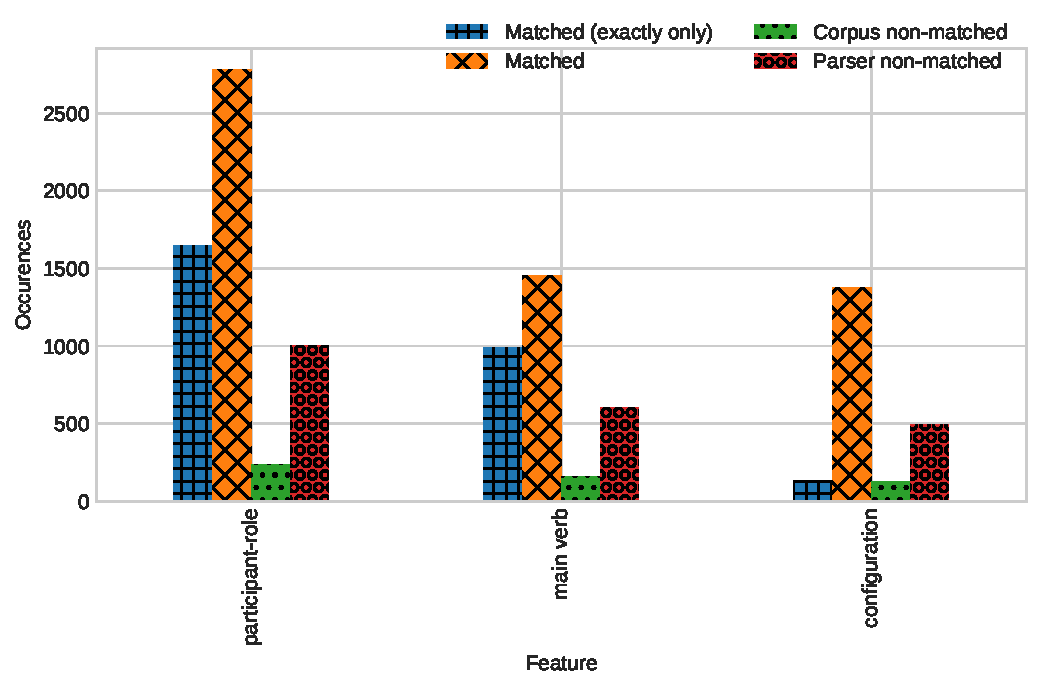
\includegraphics[width=.85\textwidth]{evaluation-results/figures/unit-elements-transitivity-data.pdf}
    \caption{Bar chart of matched and non-matched segments for the clause main Transitivity elements}
    \label{fig:unit-elements-transitivity-data}
    \end{figure}
    
    Note that in Figure \ref{fig:unit-elements-transitivity-data} the scale stretches over 2500 which reflects a much larger number of segments in the OE corpus than that available in the OCD corpus. The size, and certainly a higher quality of annotations, is reflected in the fairly uniform evaluation results. The $F_1$ (0.82), precision (0.74) and recall (0.92) scores vary very little across elements when compared to scores of the syntactic elements shown in Table \ref{tab:unit-elements-mood-combined-F1},  which vary substantially from one element to another.   

    \begin{table}[!ht]
    \centering
    \begin{tabular}{lcccccc}
    \toprule
     & \multicolumn{3}{c}{Exact match only} & \multicolumn{3}{c}{Exact and close match} \\ \cline{2-7} 
     & Precision & Recall & F1 & Precision & Recall & F1 \\ 
    \midrule
    participant-role &       0.62 &    0.88 & 0.73 &       0.74 &    0.92 & 0.82 \\
    configuration    &       0.22 &    0.52 & 0.30 &       0.74 &    0.92 & 0.82 \\
    main verb        &       0.62 &    0.86 & 0.72 &       0.71 &    0.90 & 0.79 \\ 
    \bottomrule
    \end{tabular}
    \caption{Parser accuracy statistics for the clause main Mood elements}
    \label{tab:unit-elements-transitivity-combined-F1}
    \end{table}
    
    In case of exact matches the evaluation scores are lower for the participant roles and main verbs, situating at 0.73 $F_1$ score, while the configuration accuracy plummeted to 30\%. As configurations correspond in SFG to clauses boundary establishment methodology plays a significant role in achieving exact matches. Thus the discrepancy in the $F_1$ score between exact and combined matches is explainable by a discrepancy in the clause boundaries establishment and was already addressed in Section \ref{sec:differences}. 
    
    We come to the end of the syntactic structure evaluation where I have shown that the parser generated segments exactly like those in the corpus with an accuracy of 70\% on average; and partially matching segments with an average accuracy of 80\%. The parser detects unit classes on average with 52\% accuracy for exact matches and 74\% for close matches. The Mood and Transitivity elements are detected on average with 71\% and 81\% accuracy. 
    
    A constituency parser that produces a syntactic analysis using comparable unit classes and functions (using phrase structure grammars) such as for example \citet{chen2014fast}, \citet{stern2017minimal} or \citet{kitaev2018multilingual} reached an accuracy of 95\% for English. This state of the art in parsing with other grammars reflects that there is a large space to improve the accuracy of Parsimonious Vole constituency. But it should not be separated from the context of this work which is to parse with constituency structures enriched with features from the system networks. %Next I present the evaluation of the the systemic feature selections from the MOOD and from the TRANSITIVITY system networks. 
    
\section{Evaluation of systemic feature assignment}
\label{sec:systemic-evaluation}
    
    In this section I present the evaluation results for the parser accuracy to generate the paradigmatic aspects of an SFL analysis. It constitutes an evaluation of the approach described in Chapter \ref{ch:enrichment-stage}. The discussion of evaluation results covers selection of MOOD and TRANSITIVITY features. %to clause constituents and to constituents filling the clause elements.     
    
    In this section the differentiation between exact and close matches is not considered. The reason for this is the nature of the feature selection and assignment task, which is concerned with the paradigmatic aspect of grammar. The systemic features are assigned to already formed constituent units and are not directly affected by the segmentation errors relevant at the constituent creation. 
    
\subsection{Evaluation of MOOD systemic feature assignment}
\label{sec:systemic-evaluation-MOOD}

    In this section, I present the evaluation results for the systemic selections from the MOOD system network that were assigned to clause units in the constituency structure. These features are only available in the OCD corpus annotations. The fragment of the MOOD system network that is covered by the corpus was presented in Section \ref{sec:corpus}. It is noteworthy that the parser provides with more feature selections from the MOOD system network, as described in Section \ref{sec:mood}, and that the current evaluation is limited to only what is available in the OCD corpus annotations.

    Table \ref{tab:features-mood} provides the evaluation results for each of the MOOD features grouped by system names, which are marked with capital letters. On average the parser assigns systemic features with a precision of 59\%. I do not discuss here the evaluation of each feature in part but analyse the results as a whole taking a few systems as discussion examples. A detailed discussion addressing each system in part and aiming at deeper evaluation understanding should be tackled in future work.

     \begin{table}[!ht]
        \centering
        \resizebox{0.8\textwidth}{!}{%
            \begin{tabulary}{1.1\textwidth}{@{}lCCCccc@{}}
            \toprule
             & Match & Corpus non-matched & Parser non-matched & Precision & Recall & F1 \\ \midrule
            POLARITY-TYPE &  &  &  &  &  &  \\
            positive & 485 & 125 & 55 & 0.90 & 0.80 & 0.84 \\
            negative & 57 & 10 & 70 & 0.45 & 0.85 & 0.59 \\
            VOICE-TYPE &  &  &  &  &  &  \\
            active & 553 & 102 & 68 & 0.89 & 0.84 & 0.87 \\
            passive & 11 & 11 & 28 & 0.28 & 0.50 & 0.36 \\
            FINITNESS &  &  &  &  &  &  \\
            non-finite & 99 & 19 & 38 & 0.72 & 0.84 & 0.78 \\
            finite & 526 & 33 & 554 & 0.49 & 0.94 & 0.64 \\
            NON-FINITE-TYPE &  &  &  &  &  &  \\
            perfective & 71 & 12 & 16 & 0.82 & 0.86 & 0.84 \\
            imperfective & 26 & 9 & 24 & 0.52 & 0.74 & 0.61 \\
            DEICTICITY &  &  &  &  &  &  \\
            temporal & 446 & 74 & 55 & 0.89 & 0.86 & 0.87 \\
            modal & 12 & 33 & 6 & 0.67 & 0.27 & 0.38 \\
            MOOD-ASSESSMENT-TYPE &  &  &  &  &  &  \\
            temporality & 35 & 17 & 27 & 0.56 & 0.67 & 0.61 \\
            modality & 15 & 32 & 8 & 0.65 & 0.32 & 0.43 \\
            intensity & 12 & 14 & 43 & 0.22 & 0.46 & 0.30 \\
            MOOD-TYPE &  &  &  &  &  &  \\
            indicative & 455 & 216 & 37 & 0.92 & 0.68 & 0.78 \\
            imperative & 4 & 1 & 31 & 0.11 & 0.80 & 0.20 \\
            INDICATIVE-TYPE &  &  &  &  &  &  \\
            declarative & 355 & 260 & 27 & 0.93 & 0.58 & 0.71 \\
            interrogative & 47 & 7 & 63 & 0.43 & 0.87 & 0.57 \\
            INTERROGATIVE-TYPE &  &  &  &  &  &  \\
            wh & 40 & 6 & 57 & 0.41 & 0.87 & 0.56 \\
            yes-no & 5 & 3 & 8 & 0.38 & 0.62 & 0.48 \\
            WH-SELECTION &  &  &  &  &  &  \\
            wh-subject & 9 & 3 & 7 & 0.56 & 0.75 & 0.64 \\
            wh-adjunct & 11 & 15 & 3 & 0.79 & 0.42 & 0.55 \\
            wh-complement & 8 & 0 & 62 & 0.11 & 1.00 & 0.21 \\ \bottomrule
            \end{tabulary}
        }
        \caption{The evaluation statistics available for the MOOD system network}
        \label{tab:features-mood}
    \end{table}
    
    %Table \ref{tab:features-mood} summarises the evaluation results for the MOOD system network features grouped by system name marked with capital letters.
    The order in which the features appear in Table \ref{tab:features-mood} roughly corresponds to an increase in systemic delicacy. As delicacy increases there are increasingly fewer occurrences where a system is employed. This is associated also with a decrease in the accuracy although there are multiple factors influencing this among which parser errors, corpus quality and small population size. 
    
    The precision and recall values vary quite a lot from a minimum of 11\% up to a maximum of 93\% and their harmonic mean, the $F_1$ score, between 30\% and 87\%  averaging to almost 60\%. The details can be read in Table \ref{tab:mood-accuracy}. The graphical representation of these values distribution can be seen in Figures \ref{fig:mood-precission-recall} and \ref{fig:mood-precission-f1}. A noticeable feature is the presence of two peaks in the precision and recall distributions: one around 50\% and the other one around 90\%. They translate into a similar $F_1$ distribution with peaks at 60\% and 85\%, a phenomena which I address next.

    \begin{table}[t]
        \centering
        \begin{tabular}{lccc}
            \toprule
            {} & {Precision} & {Recall} & {F1} \\ %\hline
            % feature count & 21.00 & 21.00 & 21.00 \\ \hline
            \midrule
            mean & 0.57 & 0.73 & 0.59 \\ 
            standard deviation & 0.27 & 0.18 & 0.21 \\ 
            min value & 0.11 & 0.32 & 0.20 \\ %\hline
            25\% quantile & 0.41 & 0.62 & 0.48 \\ %\hline
            50\% quantile & 0.56 & 0.80 & 0.61 \\ %\hline
            75\% quantile & 0.82 & 0.86 & 0.78 \\ %\hline
            max value & 0.93 & 1.00 & 0.87 \\ %\hline
            \bottomrule
        \end{tabular}
        \caption{Descriptive statistics of the precision, recall and F1 scores for evaluated MOOD features}
        \label{tab:mood-accuracy}
    \end{table}

    \vspace{1em}
    \noindent
    \begin{minipage}[b]{0.49\textwidth}
        \centering
        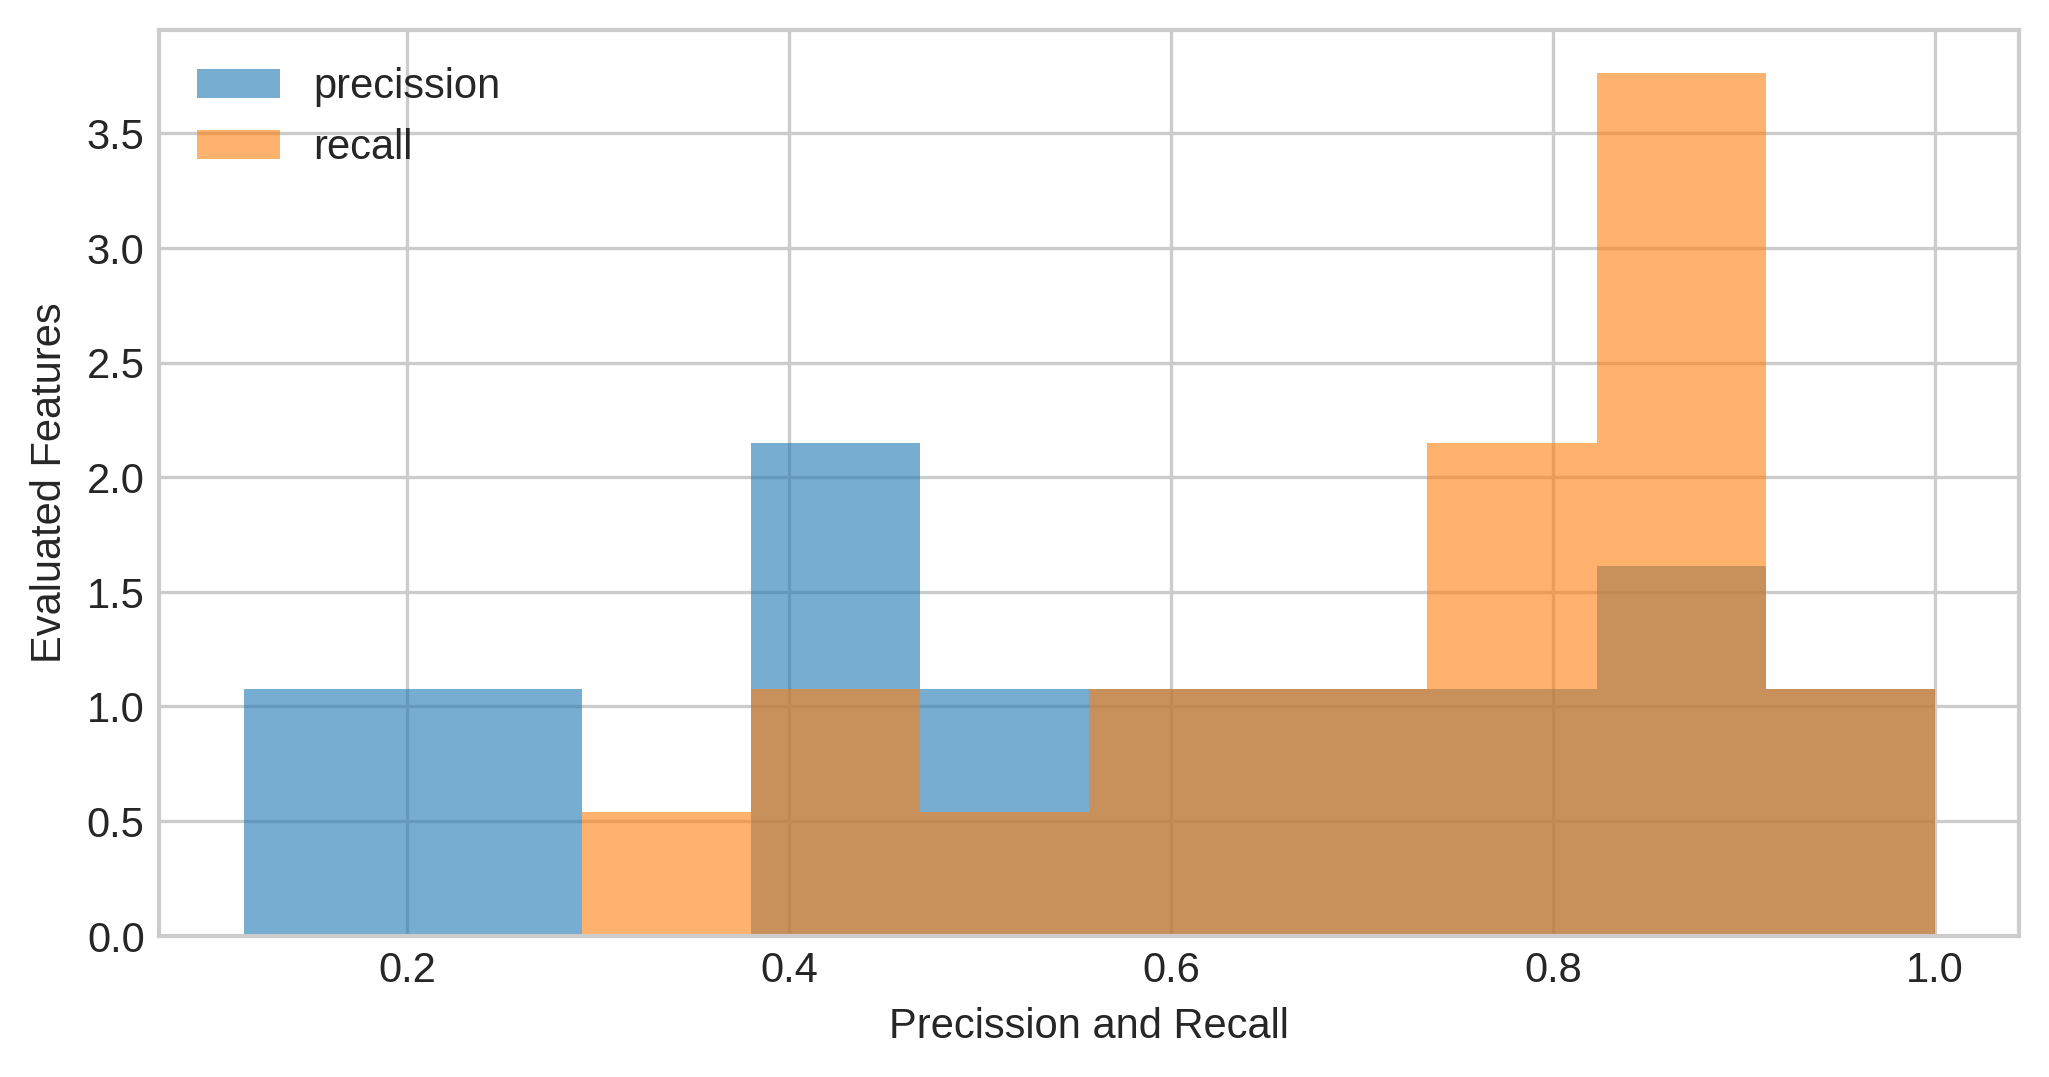
\includegraphics[width=\textwidth]{evaluation-results/figures-old/accuracy-syntactic-mood-precission-recall.png}
        \captionof{figure}{The distribution of precision and recall for evaluated MOOD features}
        \label{fig:mood-precission-recall}
    \end{minipage}
    \quad
    \begin{minipage}[b]{0.49\textwidth}
        \centering
        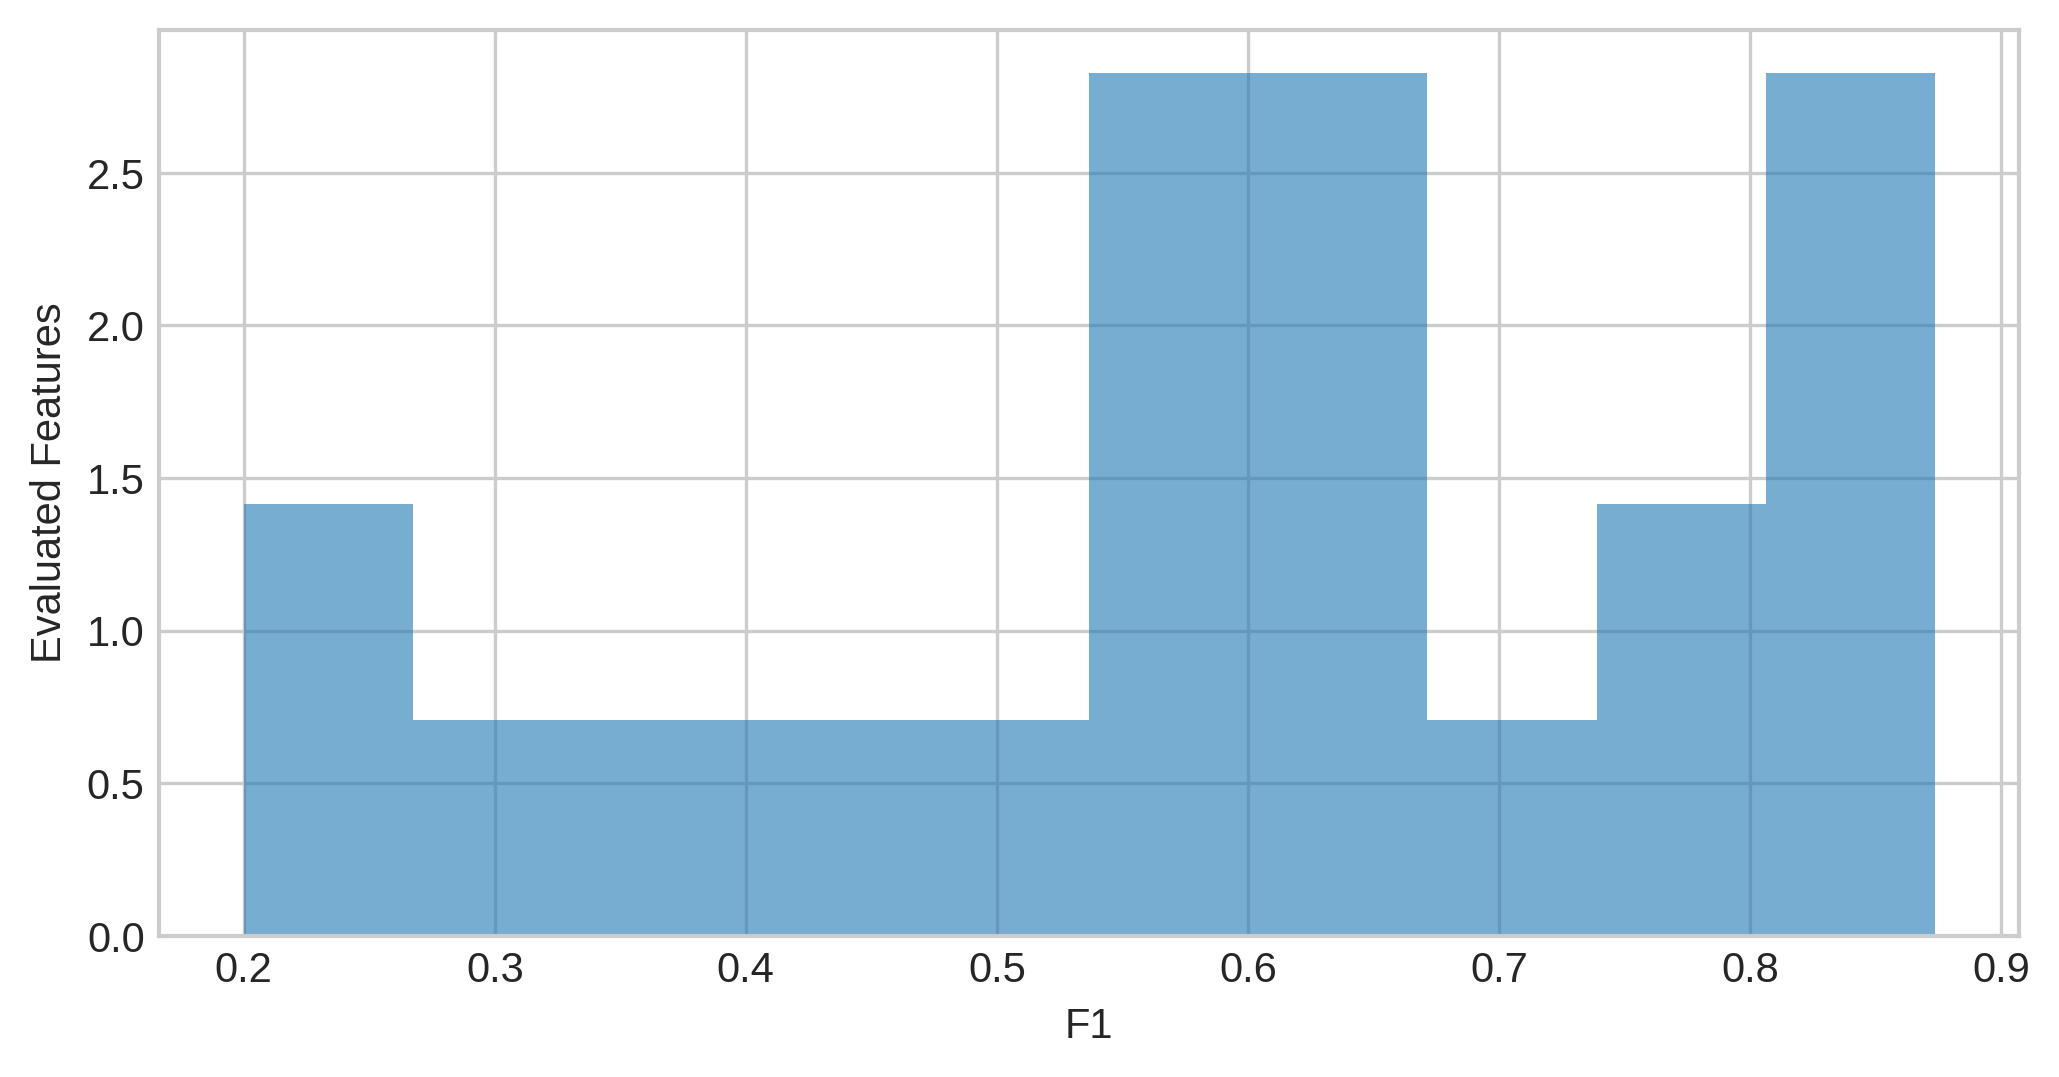
\includegraphics[width=\textwidth]{evaluation-results/figures-old/accuracy-syntactic-mood-f1.png}
        \captionof{figure}{The distribution of F1 score for evaluated MOOD features}
        \label{fig:mood-precission-f1}
    \end{minipage}
    \vspace{.5em}
    
    Within most systems, the $F_1$ scores exhibit a contrast from one feature to the other. What this possibly means is discussed in the next two cases. For example in the POLARITY-TYPE system the positive polarity feature scores 84\% accuracy while the negative one almost 60\%. As per Definition \ref{def:system}, the system features are mutually exclusive. The polarity of an English clause is positive by default unless a negation marker is found and this represents only 10\% of the clauses in  the corpus. This leads us to the hypothesis that it should be sufficient for the parser to detect one feature with a reasonably high accuracy then the converse feature should be detectable with a similar accuracy if a selection in that system is expected. Yet the current data invalidate this hypothesis as the grammar fails to represent exclusivity.
    
    In the case of the POLARITY-TYPE system, the phenomena may be explained as an incomplete parser implementation. The current version of implementation determines polarity by checking for the presence of the negation verbal marker only without considering cases of nominal and adverbial negative markers. Nonetheless a more delicate polarity testing will have to take into consideration polarity indicators from the subject, complement and adjuncts of various types that have been taken into consideration during the annotation process. An incomplete, less delicate, implementation for systemic choices is certainly a source of errors but it requires further investigation to what extent it impacts these results. %and continue testing the above hypothesis. %thus this hypothesis requires further investigation.  %The same can be expected of other systems that are reduced in delicacy 
    
    Another way to look at the high discrepancy between the feature accuracy scores can be as follows. Considering POLARITY-TYPE as example, it might be the case that most instances of positive polarity are easy to detect. But, there is a portion of cases, regardless of the polarity, that are difficult for the parser to distinguish and that the negative polarity selections fall mostly within these ambiguous cases. %It it possible that this can be generalised to other system networks and more investigation is required to pinpoint exactly how such phenomena materialise.
    
    The phenomena of unbalanced accuracy scores among siblings of the same system can be seen in multiple other cases. Let's look at the VOICE-TYPE system. The detection mechanism for VOICE-TYPE is implemented similarly to POLARITY-TYPE. The parser checks whether there is a passive order of elements in the clause, otherwise the active voice is selected.
    The detection of the active voice scores a significantly higher accuracy of 87\% than the passive one of only 36\%. There is no delicacy variation problem and still the discrepancy between the $F_1$ scores of the two features is there. But this could be explained by small sample of passive voice instances: only 22 are annotated in the corpus. 

    This section presented the evaluation results for the MOOD systemic selections. On average the parser assigns to clause constituents MOOD features with an accuracy of almost 60\%. A more thorough analysis for each system individually would indicate how to improve the current parser. At the same time the quality of the OCD annotations has not been assesses and therefore a more reliable corpus with MOOD annotations is highly desirable for a similar evaluation. %Next section provides the evaluation results for the TRANSITIVITY system network. 

    % A though for the future implementation can be to take advantage of the mutual exclusivity of system features and capitalise on the above finding, at least for the leaf systems. Taking into consideration that the score of one feature is higher, clause elements should then be provided with selections of those features only, while the complement features, which score low in this evaluation should remain unassigned. This means that only features that can be provided with high confidence (using $F_1$ score as a measure of that) shall be assigned. Then an additional process can be implemented to select the remaining unassigned features. 
    
    
\subsection{Evaluation of TRANSITIVITY systemic feature assignment}
\label{sec:systemic-evaluation-TRANSITIVITY}
    
    In this section I present the evaluation of the TRANSITIVITY system network. As was explained in Section \ref{sec:corpus} above, the OE corpus contains annotations covering only a fragment of the TRANSITIVITY system, which is depicted in Figure \ref{fig:transitivity-simplified}. The full Cardiff TRANSITIVITY system network was presented in Figure \ref{fig:cardiff-transitivity} in Chapter \ref{ch:the-grammar}. The parser provides more feature selections than those available in the corpus, which are described in Section \ref{sec:transitivity}, but the current evaluation is limited to only what is available in the corpus.
    
    Cardiff Transitivity analysis is semantic in nature and poses challenges in meaning selection beyond constituent class or function. The approach of assigning this sort of features was explained in Chapter \ref{ch:enrichment-stage}. Here I would like to remind about an important aspect of this approach that impacts the evaluation results, explaining in some cases abnormally high recall rates.
    
    In the grammar, described in Chapter \ref{ch:the-grammar}, a clause can be assigned a single process configuration and the participant constituents can take only one role each. In the semantic role labelling task the situation is similar: a clause takes one semantic frame and each constituent only one semantic label. This means that a parser shall produce as output one semantic configuration that fits best the text. 
    
    The approach implemented in the Parsimonious Vole parser is such that it does not always provide a single semantic configuration. Instead, it generates one or several possible configurations for each clause instead of providing exactly a one. The reason for this is the mechanism by which semantic analysis is done. The constituency structure is tested against a set of semantic graph patterns and the matching patterns enrich the constituency structure with semantic features immediately. In some cases more than one pattern matches the constituency structure leading to enrichment by multiple graph patterns, which is not entirely correct. 
    
    Multiple features assignment from the same system, however, are represented as disjunctive sets in the constituency structure which ought to be interpreted as alternating possibilities rather than actual assignments. This interpretations was explained in Chapter \ref{ch:data-structures} when the disjunctive sets were introduced.
    
    Intuitively, this should reduce accuracy on all the elements but the effects are mostly manifested at the level of participant roles as will be described below. First, let's discuss the evaluation results for the process types, which are provided in Table \ref{tab:features-transitivity}, and after, we will turn to the evaluation of participant roles.
    
    \begin{table}[!ht]
    \centering
    \resizebox{0.8\textwidth}{!}{%
        \begin{tabulary}{1.1\textwidth}{@{}lCCCccc@{}}
        \toprule
         & Match & Corpus non-matched & Parser non-matched & Precision & Recall & F1 \\ \midrule
        PROCESS-TYPE &  &  &  &  &  &  \\
        mental & 277 & 231 & 87 & 0.76 & 0.55 & 0.64 \\
        relational & 338 & 297 & 174 & 0.66 & 0.53 & 0.59 \\
        influential & 38 & 51 & 62 & 0.38 & 0.43 & 0.40 \\
        action & 170 & 231 & 352 & 0.33 & 0.42 & 0.37 \\
        event-relating & 1 & 28 & 0 & 1.00 & 0.03 & 0.07 \\
        RELATIONAL-TYPE &  &  &  &  &  &  \\
        attributive & 169 & 239 & 107 & 0.61 & 0.41 & 0.49 \\
        directional & 30 & 13 & 127 & 0.19 & 0.70 & 0.30 \\
        locational & 39 & 20 & 207 & 0.16 & 0.66 & 0.26 \\
        matching & 2 & 0 & 69 & 0.03 & 1.00 & 0.05 \\
        MENTAL-TYPE &  &  &  &  &  &  \\
        three-role-cognition & 45 & 51 & 34 & 0.57 & 0.47 & 0.51 \\
        two-role-cognition & 95 & 102 & 86 & 0.52 & 0.48 & 0.50 \\
        two-role-perception & 13 & 12 & 102 & 0.11 & 0.52 & 0.19 \\
        three-role-perception & 0 & 2 & 6 &  &  &  \\
        desiderative & 0 & 0 & 81 &  &  &  \\
        emotive & 0 & 0 & 87 &  &  & \\ \bottomrule
        \end{tabulary}
    }
    \caption{The evaluation statistics available for the PROCESS-TYPE system and few of its subsystems from the TRANSITIVITY system network}
    \label{tab:features-transitivity}
    \end{table}
    
    In Table \ref{tab:features-transitivity} \textit{mental} and \textit{relational} processes are the ones with highest $F_1$ scores: 0.64 and 0.59. They are followed by \textit{influential} and \textit{action} process types while results for the \textit{event-relating} are not conclusive because of the very small number of occurrences in the dataset. 
    % This can be read in Table \ref{tab:features-transitivity} where the number of matched segments is higher than the number of non matched corpus or parser segments. 
    Note that considerable volume of annotations for process type sub-types are provided for mental and relational processes as explained in \citet[153-155]{schulz2015me}.
    
    Among the \textit{mental} processes, \textit{two-role-cognition} and \textit{three-role-cognition} are parsed with the highest accuracy of 51\% and 50\% correspondingly; whereas among \textit{relational} ones the \textit{attributive} process type scores the highest, 49\% while the rest of them score much lower. This can be seen also in the higher number of  non-matched segments for each process type for every feature.
    
    \begin{table}[!ht]
    \centering
    \begin{tabular}{lccc}
        \toprule
        {} & {Precision} & {Recall} & {F1} \\ %\hline
        \midrule
        mean & 0.35 & 0.48 & 0.36 \\
        standard deviation & 0.32 & 0.26 & 0.19 \\
        min value & 0.00 & 0.00 & 0.05 \\
        25\% quantile & 0.07 & 0.42 & 0.24 \\
        50\% quantile & 0.33 & 0.48 & 0.39 \\
        75\% quantile & 0.59 & 0.55 & 0.51 \\
        max value & 1.00 (0.76) & 1.00 (0.70) & 0.64 \\
        \bottomrule
    \end{tabular}
    \caption{Descriptive statistics of the precision, recall and F1 scores for evaluated TRANSITIVITY features}
    \label{tab:transitivity-accuracy}
    \end{table}
    
    Looking at the entire set of evaluation results for process types, the precision and recall values vary quite a lot from a minimum of 3\% up to a maximum of 100\% and the $F_1$ score, between 7\% and 64\%  averaging to 41\%. The summary of the descriptive statistics can be read in Table \ref{tab:transitivity-accuracy}. The maximum of 100\% precision is a bit unfortunate because there is one instance of the event-relating process found by the parser which also failed to find the other 28 thus the recall of 3\% only. Hence, I decided to ignore this value and use the next maximum which is 76\% corresponding to the mental process types. A similar case of 100\% is for recall of the matching process type which was provided only two times in the corpus, but the parser generated 67 different instances of it. Therefore, I consider the next maximum recall value, 70\%  for the directional process type. 
    
    Next, I provide an analysis of the evaluation data indicating a potential relation between the increase in the delicacy and effect it has on the parser accuracy. The accuracy of mental process detection is 64\% whereas the average accuracy for the mental sub-types (cognition, perception, desiderative and emotive) is 40\%. The same holds for relational process whose accuracy is 59\%, whereas the average of its sub-types (attributive, directional, locational, matching) is only 26\%. I start by comparing the number of mental and relational segments to the sum of mental sub-type segments and sum of relational sub-type segments correspondingly. 
    
   \begin{table}[!ht]
    \noindent
    \resizebox{0.98\linewidth}{!}{%
     \begin{minipage}[t]{0.495\textwidth}
         \centering
         \resizebox{0.995\textwidth}{!}{%  
             \begin{tabulary}{1.2\textwidth}{|C|c|c|c|}
                 \hline
                 \textbf{Features} & \textbf{Manual} & \textbf{Parse} & \textbf{/} \\ \hline
                 mental & 508 & 364 & \textbf{0.72} \\ \hline
                 mental sub-types (sum of) & 320 & 549 & \textbf{1.72} \\ \hline
                 \textbf{/} & \textbf{0.63} & \textbf{1.51} &  \\ \hline
             \end{tabulary}
         }
         \caption{The ratios between \textit{mental} segments and the sum of mental sub-type segments}
         \label{tab:ratios-mental}
     \end{minipage}%
     \quad
     \begin{minipage}[t]{0.495\textwidth}
         \centering
         %    \begin{table}[!ht]
         \resizebox{0.995\textwidth}{!}{%  
             \begin{tabulary}{1.2\textwidth}{|C|c|c|c|}
                 \hline
                 \textbf{Features} & \textbf{Manual} & \textbf{Parse} & \textit{\textbf{/}} \\ \hline
                 relational & 635 & 512 & \textbf{0.8} \\ \hline
                 relational sub-types (sum of) & 512 & 750 & \textbf{1.47} \\ \hline
                 \textit{\textbf{/}} & \textbf{0.8} & \textbf{1.47} &  \\ \hline
             \end{tabulary}
         }
         \caption{The ratios between \textit{relational} segments and the sum of mental sub-type segments}
         \label{tab:ratios-relational}
         %    \end{table}
     \end{minipage}
     }
    \end{table}
    
    Table \ref{tab:ratios-mental} and \ref{tab:ratios-relational} contain four frequency counts and four ratios. The total number of segments available in the corpus and produced by the parser are provided by column and the features are provided in rows. On the bottom and right sides of the table two pairs of ratios between frequency numbers are provided. 
    
    Next, I discuss only the case of the mental process type (see Table \ref{tab:ratios-mental}) because the values of the ratios are very similar and the same holds for relational processes. Perhaps this holds for other process types but we still lack data for testing this hypothesis further. 
    
    The first pair of ratios, provided in the lowest row, compare the number of segments with \textit{mental} feature to the sum of segments with any sub-type of \textit{mental} feature (i.e.  \textit{cognition}, \textit{perception}, \textit{emotive}, etc.). This ratio measures how well the feature dependencies are preserved across delicacy levels. The second pair of ratios, provided in the last column, compares the number of segments provided by the parser to that available in the corpus for both the mental feature and the sum of its sub-types.
    
    Table \ref{tab:ratios-mental} shows that in the corpus the number of segments with the \textit{mental} feature is almost one fourth higher than what the parser provides (72 \%). This result means that probably not all the instances of a mental process have been detected by the parser (i.e. 28\% undetected). The same comparison ran on the sub-types of \textit{mental} process shows diametrically opposite results, i.e. three quarters more parser results than in the corpus (172\%) which is an indication of multiple false positives. A possible explanation is the correlation between increase in delicacy and uncertainty, i.e. the more delicate features are less precise in the parser results. As mentioned in the beginning of this section, uncertainty, in this case, is manifested as excessive production of process types represented in disjoint sets of possible options. Currently, no ranking mechanism is put in place that would suggest the best option from the candidate ones. Hence, the parser provides multiple feature selections from the same system (in this case MENTAL-TYPE) for a constituent, whereas there should be a single one. In the future this needs to be addressed by introducing a discrimination mechanism. It could, for instance, collect all the possible matches first and then only the most suitable to be assigned to the constituent unit, possibly by using frequencies available from a corpus annotations like OE or other sources.
    
    If we look again at Table \ref{tab:ratios-mental} and compare the number of all mental sub-type occurrences to the number of mental type occurrences, then we see that the ratio is quite low (63\%). As the delicacy of the features increases fewer of these features are provided in the corpus. This is a direct manifestation of difficulty in annotating with ever more delicate features. This ratio, therefore, measures the degree of incompleteness at this level of delicacy. Comparing the same ratio for the parser generated segments we notice an opposite result (151\%). This ratio represents a measurement of the noise (false positives) produced by the parser due to an increase in uncertainty resulting from advancing to a more delicate system in the network (as was already explained above). 
    
    \begin{table}[!t]
    \centering
    % \resizebox{0.8\textwidth}{!}{%
        \begin{tabulary}{0.8\textwidth}{@{}lCCCccc@{}}
        \toprule
        & Match & Corpus non-matched & Parser non-matched & Precision & Recall & F1 \\ 
        \midrule
        emoter & 91 & 70 & 57 & 0.61 & 0.57 & 0.59 \\
        phenomenon & 359 & 223 & 294 & 0.55 & 0.62 & 0.58 \\
        carrier & 267 & 263 & 244 & 0.52 & 0.50 & 0.51 \\
        cognizant & 82 & 84 & 104 & 0.44 & 0.49 & 0.47 \\
        agent & 267 & 210 & 428 & 0.38 & 0.56 & 0.46 \\
        possessed & 71 & 24 & 155 & 0.31 & 0.75 & 0.44 \\
        attribute & 162 & 241 & 170 & 0.49 & 0.40 & 0.44 \\
        affected & 93 & 70 & 663 & 0.12 & 0.57 & 0.20 \\
        \bottomrule
        \end{tabulary}
    % }
    \caption{The evaluation statistics available for the PARTICIPANT-ROLE-TYPE system from the TRANSITIVITY system network}
    \label{tab:features-participant-role-restricted}
    \end{table}
    
    So far we have discussed evaluation for the process types and now let's turn attention towards the feature assignments from the PARTICIPANT-ROLE-TYPE system. Table \ref{tab:features-participant-role-restricted} presents the data considered for this evaluation along with the precision, recall and $F_1$ score for each participant role sorted according to $F_1$ score in descending order. 
    
    \begin{table}[!b]
    \centering
    \begin{tabular}{lccc}
        \toprule
        {} & {Precision} & {Recall} & {F1} \\ %\hline
        \midrule
        mean & 0.43 & 0.56 & 0.46 \\
        standard deviation & 0.16 & 0.10 & 0.12 \\
        min value & 0.12 & 0.40 & 0.20 \\
        25\% quantile & 0.37 & 0.50 & 0.44 \\
        50\% quantile & 0.46 & 0.56 & 0.46 \\
        75\% quantile & 0.53 & 0.58 & 0.53 \\
        max value & 0.61 & 0.75 & 0.59 \\
        \bottomrule
    \end{tabular}
    \caption{Descriptive statistics of the precision, recall and F1 scores for evaluated PARTICIPANT-ROLE features}
    \label{tab:features-participant-role-accuracy}
    \end{table}
    
    In this evaluation only the participant roles that appear at least 100 times in the corpus are considered. This restriction is inherited from \citet[160-162]{schulz2015me} study on the OE corpus. %The entire set of evaluation results for participant roles is provided in Table \ref{tab:features-participant-role} in Appendix \ref{ch:evaluation-data}. 
    
    The evaluation results for considered set of participant roles is summarised in Table \ref{tab:features-participant-role-accuracy}. The precision varies from 12\% to 61\% with an average of 43\%, and the recall varies between 40\% and 75\% with an average of 56\%. The data is characterised by lower precision and higher recall, which is directly reflected in the $F_1$ score averaging to 46\%. 
    
    The distribution of precision, recall and $F_1$ scores can be seen in Figures \ref{fig:participant-role-precission-recall} and \ref{fig:participant-role-precission-f1}. The noticeable feature is the peak of precision near the 0.5 mark and that of recall around 0.6. They translate into $F_1$ distribution as three groups: a small first group near the minimum pole, formed by the affected feature; a second tall tower at 45\% accuracy formed by cognizant, agent, possessed and attribute features; and a third group around 55\% accuracy on the right side of the graph formed by the emoter, phenomenon and carrier.
    
    \vspace{1em}
    \noindent
    \begin{minipage}[b]{0.49\textwidth}
        \centering
        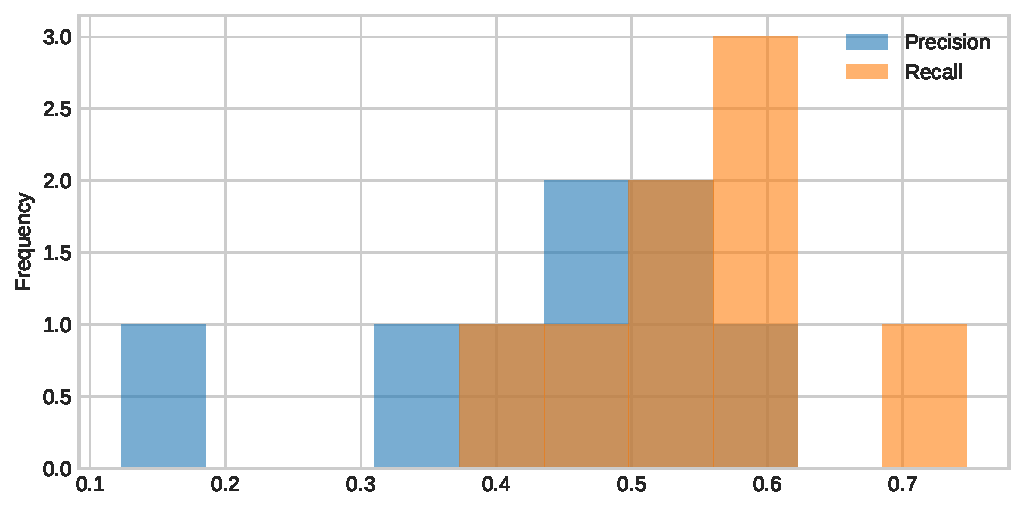
\includegraphics[width=\textwidth]{evaluation-results/figures/PARTICIPANT-ROLE-distribution-PR-10.pdf}
        \captionof{figure}{The distribution of precision and recall for evaluated PARTICIPANT-ROLE features}
        \label{fig:participant-role-precission-recall}
    \end{minipage}
    \quad
    \begin{minipage}[b]{0.49\textwidth}
        \centering
        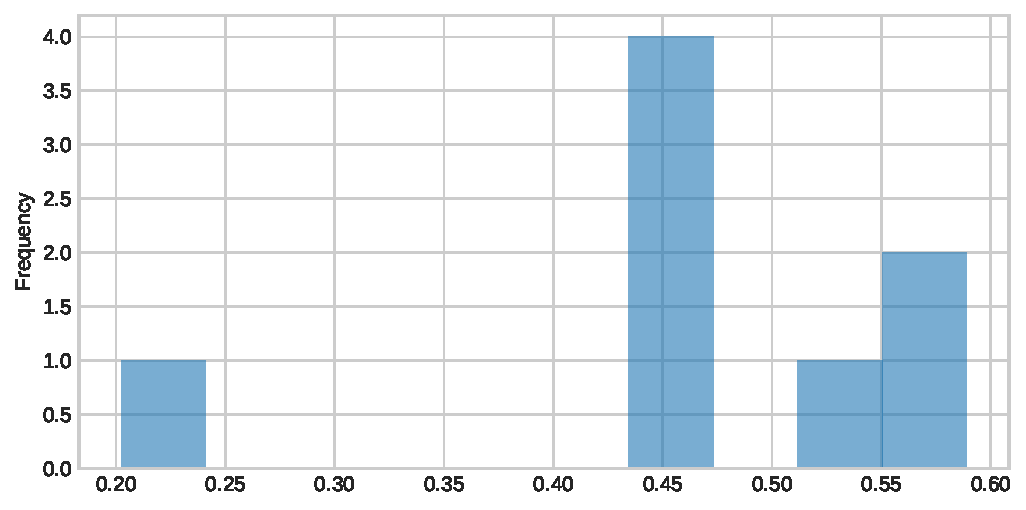
\includegraphics[width=\textwidth]{evaluation-results/figures/PARTICIPANT-ROLE-distribution-F1-10.pdf}
        \captionof{figure}{The distribution of F1 score for evaluated PARTICIPANT-ROLE features}
        \label{fig:participant-role-precission-f1}
    \end{minipage}
    \vspace{1em}
    
    In Table \ref{tab:features-participant-role-restricted} a suite of eight features have $F_1$ scores descending from almost 60\% to 44\%. The affected features follow with half of the previous (20\%). As the accuracy decreases we can notice that few features display high recall especially in the case of the \textit{affected} feature, which spiked to 600\% the number of matched segments. This is a direct manifestation of the assignment of multiple roles to one participant by multiple graph patterns (for the reasons explained in the beginning of this section). This abnormally high number of participants produced by the parser must be addressed in future work starting with an investigation of the Transitivity graph patterns generated from the PTDB, in particular for the  affected feature. The next section will conclude this evaluation chapter.

    % From the data presented in Table \ref{tab:features-participant-role} we can conclude that only the first one third of the participant roles can be considered usable with a reasonable level of confidence. It also shows a serious lack of data for the lower one third of the participant roles, which is directly reflected in low precision scores. A hypothesis that I put forward here is that in a larger corpus, with broader coverage over the participant roles, the scores for the rare features would improve considerably compared to this results. 
    
    % The compound roles such as affected-carrier, affected-possessed, agent-perceiver etc. have scored very low accuracy especially if compared to their simple counter parts. For example carrier role is detected with an accuracy of 51\% and affected role with  20\% while the compound role with very low accuracy of only 7\%. This indicates that in future work the way compound roles are assigned by the parser and how these assignments are evaluated should be rethought and a different approach taken.  
    

\section{Summary}
\label{sec:evaluation-discussion}
    
    In this chapter we have discussed how the empirical evaluation of Parsimonious Vole parser has been conducted. The stage is set through a general presentation of the corpora and what the task at hand is, i.e. identifying and comparing segments available in the corpus annotations to those generated automatically by the parser. The accuracy is determined by the parser ability to generate identical or partially overlapping segments to those in the corpus.
    
    Section \ref{sec:corpus} presented the OCD and OE corpora, which are employed in the current evaluation exercise. The OCD corpus is used for measuring the accuracy of the constituency structure produced by the parser and MOOD feature assignments to clause units. The OE corpus is used to evaluate TRANSITIVITY feature assignments to configuration and participant constituents. The parser output does not follow entirely the annotation methodology used in annotation of the corpus, therefore there are a few differences to account for, which were explained in Section \ref{sec:differences}. 
    
    Section \ref{sec:evaluation-methodology} explained how the current evaluation is performed. It starts by defining what is evaluated, i.e. labelled segments, then explains how corpus annotations and parser output are represented as sets of segments, and finally presents how these batches are compared to one another deriving from that parser accuracy measurements and how the measurement data is structured. The alignment algorithm, presented in the same section, takes into consideration not only the exact but also the partial matches. %The results are discussed in the next section. 
    
    The following two sections, \ref{sec:syntactic-evaluation} and \ref{sec:systemic-evaluation}, presented the evaluation data and discussed the findings. The evaluation of the segmentation task revealed that 71\% of the segment have identical spans and that 83\% of the segments are identical or shifted slightly (up to 5 characters). There are several ways to measure distance and among the tested ones the most significant were the geometric distance and the WindowDiff distance, while the other distances were omitted from the discussion because they strongly correlated to one of these two. 
    %The results of evaluating constituency structure are as follows. 
    The results showed that, the parser assigns classes to the constituent units with an accuracy of 74\%; furthermore, clause main Mood elements are assigned with an accuracy of 71.2\% while the Transitivity elements with an accuracy of 81\%. 
    
    The current parser accuracy is similar to that reported by \citet{Souter1996}, i.e. 76\% for the first six solutions. This score, however, means that the correct parse tree is found among the first six ones generated by the parser, which is a non practical approach. 
    
    \citet{ODonoghue91}, using Vertical Strip Parsing, scored 81\%, which is about 5\% higher than that of the current parser. However his evaluation was based on a much narrower coverage of English than that found in the OE and OCD corpora because he used an extract from the COMMUNAL NL generator GENESYS PG 1.5 version.
    
    When it comes to evaluating the accuracy of systemic assignments, the measured accuracy varies across delicacy levels and between sibling features within the same system, which was addressed for MOOD and especially for TRANSITIVITY in Section \ref{sec:systemic-evaluation}.
    The accuracy measurements are provided for a fraction of the MOOD system network and a fraction of TRANSITIVITY system network. This is based on their availability in the corpus annotations, which was described in Section \ref{sec:corpus}. The features from the MOOD system network are assigned, on average, with an accuracy of 59\%. The accuracy of TRANSITIVITY system network was measured for the PROCESS-TYPE system and the PARTICIPANT-ROLE-TYPE system separately. The accuracy of the former, on average, is 36\% and the latter, on average, is 46\%. 
    
    The present evaluation results are significant in at least two major respects. First, the parser overall accuracy is comparable to or slightly lower than the accuracy achieved by previous attempts of generating SFL constituency structures e.g. 76\% by \citet{Souter1996} and 81\% by \citet{ODonoghue91}.
    Moreover, the parser produces feature rich output which sets apart Parsimonious Vole from other parsers. The features in the produced output could be already considered useful in some practical situations where identifying in text Mood or Transitivity features is needed. 
    Second, this study shows which areas are in need of improvement and provides some hints on what could be the reason for the poor performance. Also, this evaluation is the first one and constitutes the baseline for further incremental developments.
    
    Even if it is completely separate action, this evaluation can be useful for further corpus improvements as well. When I mention corpus improvement I bear in mind the OCD corpus in particular, which needs to be annotated by at least one more annotator and tested for reliability. In addition, the corpora size is fairly small and many systemic features are under-represented or missing completely as is the case, for example, of event-relating, environmental, action sub-types and other processes. It would be desperately necessary but quite unlikely to happen \citep[33]{mcenery2006corpus} to extend the corpus annotation to include more delicate MOOD and TRANSITIVITY features. This will enable the study of how the features vary and how accurately the parser detects them. 
    
    The next chapter concludes the work done so far providing new ideas and setting a tone for what needs to be done in future work to improve the current results.